\documentclass[british,titlepage]{ntnuthesis}

\usepackage{tikz} \usetikzlibrary{arrows, backgrounds, external, fit, positioning, shapes, trees}
\usepackage{rotating}
\usepackage{multirow}
\usepackage{longtable}
\usepackage{lscape}

\title{Enterprise architecture to support learning in and across cities}
\shorttitle{EA to support learning in cities}
\author{Eldar Hauge Torkelsen}
\shortauthor{Torkelsen, Eldar H.}
\date{2021/06/22}

% Reuse tikz pictures instead of recompile
%\tikzexternalize[prefix=tikz/]

\addbibresource{thesis.bib}


% From https://www.overleaf.com/learn/latex/Glossaries

\makeglossaries % Prepare for adding glossary entries

\iffalse
\newglossaryentry{latex}
{
        name=latex,
        description={Is a mark up language specially suited for
scientific documents}
}

\newglossaryentry{bibliography}
{
        name=bibliography,
        plural=bibliographies,
        description={A list of the books referred to in a scholarly work,
typically printed as an appendix}
}

\newglossaryentry{maths}
{
    name=mathematics,
    description={Mathematics is what mathematicians do}
}
\fi

% --------------------
% ----- Glossary -----
% --------------------
\newglossaryentry{boundary object}
{
    name={boundary object},
    description={Objects that contain information used by multiple communities that might be interpreted differently from one community to another}
}
\newglossaryentry{spss}{
    name={SPSS},
    description={Software for statistical analysis}
}
\newglossaryentry{ict ecosystem}{
    name={\gls{ict} ecosystem},
    description={An \gls{ict} system and the systems it interacts with.}
}

\newglossaryentry{the open group}{
    name={The Open Group},
    description={A global consortium creating open technology standards.}
}
% --------------------
% ----- Acronyms -----
% --------------------
\iffalse
\newacronym{phd}{PhD}{philosophiae doctor}
\newacronym{CoPCSE}{CoPCSE@NTNU}{Community of Practice in Computer ScienceEducation at NTNU}
\newacronym{gcd}{GCD}{Greatest Common Divisor}
\fi

\newacronym{adm}{\gls{togaf} ADM}{\gls{togaf} Architecture Development Method}
\newacronym{api}{API}{Accessible Programming Interface}
\newacronym{ea}{EA}{Enterprise Architecture}
\newacronym{eaf}{EAF}{Enterprise Architecture Framework}
\newacronym{ict}{ICT}{Information and Communications Technology}
\newacronym{it}{IT}{Information technology}
\newacronym{ka}{KA}{Knowledge Architecture}
\newacronym{km}{KM}{Knowledge management}
%\newacronym{km}{KM}{Knowledge Modelling} 
\newacronym{kpi}{KPI}{Key Performance Indicator}
\newacronym{mom}{MOM}{Message-oriented middleware}
\newacronym{mvc}{MVC}{Model View Controller}
\newacronym{ntnu}{NTNU}{Norwegian University of Science and Technology}
\newacronym{scis}{SCIS}{EU Smart Cities Information System}
\newacronym{tam}{TAM}{Technology Acceptance Model \cite{davis1989perceived}}
\newacronym{togaf}{TOGAF}{The Open Group Architecture Framework}
\newacronym{ocl}{OCL}{Object Constraint Language}
\newacronym{ui}{UI}{User Interface}
\newacronym{uml}{UML}{Unified Modeling Language}
\newacronym{uri}{URI}{Uniform Resource Identifier}
\newacronym{url}{URL}{Uniform Resource Locator}
\newacronym{emaas}{EMaaS}{Electric Mobility as a Service}
\newacronym{nsd}{NSD}{Norwegian Centre for Research Data}
 % add glossary and acronym lists before document

% Configure package settings
\makeatletter
\pgfdeclareshape{api}{
    \savedanchor{\centerpoint}{
        \pgfpointorigin
    }
    %\savedanchor{owner}{
    %    \centerpoint
    %    \pgf@x=-2*\ht\pgfnodeparttextbox
    %}
    %\savedanchor{user}{
    %    \centerpoint
    %    
    %}

    \anchor{west}{      % Something is causing the anchor to be at origin
       \centerpoint
       %\advance \pgf@x by -2*\ht\pgfnodeparttextbox
       %\pgfpoint{\pgf@x}{\pgf@y}
    }
    \anchor{east}{      % Something is causing the anchor to be at origin
        \centerpoint \pgf@xa=\pgf@x \pgf@ya=\pgf@y
        %\pgfmathsetlength\pgf@x{2.5*\ht\pgfnodeparttextbox}
    }
    \anchor{center}{   
        \centerpoint
    }

    \anchor{text}{
        \centerpoint
        \pgf@x=+\ht\pgfnodeparttextbox%
        \pgf@y=-2\ht\pgfnodeparttextbox
    }
    
    \backgroundpath{
        \centerpoint \pgf@xa=\pgf@x \pgf@ya=\pgf@y
        \pgfpathmoveto{\pgfpoint{\pgf@xa}{\pgf@ya}}
        \pgfpathcircle{
            \pgfpoint{\pgf@xa}{\pgf@ya}
        }{
            \ht\pgfnodeparttextbox
        }
        \pgfpathmoveto{
            \pgfpoint{\pgf@xa-1.0*\ht\pgfnodeparttextbox}{\pgf@ya+1.5*\ht\pgfnodeparttextbox}
        }
        \pgfpatharc{90}{-90}{1.5*\ht\pgfnodeparttextbox}
        \pgfpathmoveto{
            \pgfpoint{-1*\ht\pgfnodeparttextbox}{\pgf@ya}
        }
        \pgfpathlineto{
            \pgfpoint{-2*\ht\pgfnodeparttextbox}{\pgf@ya}
        }
        \pgfpathmoveto{
            \pgfpoint{1.5*\ht\pgfnodeparttextbox}{\pgf@ya}
        }
        \pgfpathlineto{
            \pgfpoint{2.5*\ht\pgfnodeparttextbox}{\pgf@ya}
        }
        
    }
}
\makeatother
\begin{document}

\tikzset{%
  % Specifications for style of nodes:
            base/.style = {rectangle, draw=black,
                           minimum width=4cm, minimum height=1cm,
                           text centered},
  activityStarts/.style = {base, rounded corners, fill=blue!30},
       startstop/.style = {base, rounded corners, fill=red!30},
    activityRuns/.style = {base, rounded corners, fill=green!30},
         process/.style = {base, rounded corners, minimum width=2.5cm, fill=orange!15,
                           font=\ttfamily},
    objective/.style    = {base, draw=black, fill=blue!30},
    activity/.style     = {base, rounded corners, fill=red!10},
    output/.style        = {base},
}

\chapter*{Acknowledgement}
Thanks to my supervisor Sobah Abbas Petersen and co-supervisor Anthony Junior Bokolo for guidance and good feedback. Thanks to Mohammad Ali Kohansal, Markus Helfert and Zohreh Pourzolfaghar for giving feedback on the questionnaire draft. Thanks to those whom helped with model evaluation, and thanks to those in the +CityxChange project for providing a platform that was invaluable for my research. 
\chapter*{Abstract}
\iffalse
The \texttt{ntnuthesis} document class is a customised version of the standard \LaTeX{} \texttt{report} document class. It can be used for theses at all levels – bachelor, master and PhD – and is available in English (British and American) and Norwegian (Bokmål and Nynorsk). This document is ment to serve (i) as a description of the document class, (ii) as an example of how to use it, and (iii) as a thesis template.
\fi

Smart city development efforts have met hindrances when trying to replicate solutions in other cities. This thesis studies the more general approach of learning and knowledge transfer from the development effort, across cities. It specifically looks at the role of Enterprise Architecture to facilitate learning and knowledge transfer in smart city projects. A literature review and a survey have been conducted to answer the questions of how Enterprise Architecture currently supports learning and how it can be improved in that regard. Further, it applies its findings on The Enterprise Architecture framework used in the +CityxChange project and evaluates the proposed changes with an expert evaluation. It concludes that  the complexity and terminology used in the Enterprise Architecture framework are limiting factors for its use in learning.
\chapter*{Sammendrag}
\iffalse
Dokumentklassen \texttt{ntnuthesis} er en tilpasset versjon av \LaTeX' standard \texttt{report}-klasse. Den er tilrettelagt for avhandlinger på alle nivåer – bachelor, master og PhD – og er tilgjengelig på både norsk (bokmål og nynorsk) og engelsk (britisk og amerikansk). Dette dokumentet er ment å tjene (i) som en beskrivelse av dokument\-klassen, (ii) som et eksempel på bruken av den, og (iii) som en mal for avhandlingen.
\fi

Smart by utbyggings prosjekt har møt hindinger når de prøver å gjenskape løsninger i andre byer. Denne oppgaven studerer den mer generelle tilnærmingen av å lære og videreføre kunskap fra utbyggings prosjektene, på tvers av byer. Den ser mer spesifikt på rollen til Virksomhets-arkitektur for å fremme læring og kunskaps videreføring i smart by prosjekt. En Literatur analyse og en spørre undersøkelse ble utført for å svare på spørsmålene om hvordan Virksomhets-arkitektur blir brukt for å hjelpe med læring og hvordan det kan blir forbedret for det formålet. I tilleg brukes funnene på Virksomhets-arkitektur rammeverket som blir brukt i +CityxChange prosjektet og evaluerer de foreslåtte endringene med en ekspert evaluering. Oppgaven konkluderer at kompleksitet og terminologien brukt i Virksomhets-arkitektur rammeverket er begrensende faktorer for dens bruk innenfor læring. 

\tableofcontents
\listoffigures
\listoftables
\lstlistoflistings

\printglossary[type=\acronymtype] % Print acronyms
\printglossary                    % Print glossary

\chapter{Introduction}
\label{chap:introduction}
\iffalse %-----------------------------------------------------------------------------------
Over the years, several thesis templates for \LaTeX{} have been developed by different groups at NTNU. Typically, there have been local templates for given study programmes, or different templates for the different study levels – bachelor, master, and \acrshort{phd}.\footnote{see, e.g., \url{https://github.com/COPCSE-NTNU/bachelor-thesis-NTNU} and \url{https://github.com/COPCSE-NTNU/master-theses-NTNU}}

Based on this experience, the \acrfull{CoPCSE}\footnote{\url{https://www.ntnu.no/wiki/display/copcse/Community+of+Practice+in+Computer+Science+Education+Home}} is hereby offering a template that should in principle be applicable for theses at all study levels. It is closely based on the standard \LaTeX{} \texttt{report} document class as well as previous thesis templates. Since the central regulations for thesis design have been relaxed – at least for some of the historical university colleges now part of NTNU – the template has been simlified and put closer to the default \LaTeX{} look and feel.

The purpose of the present document is threefold. It should serve (i) as a description of the document class, (ii) as an example of how to use it, and (iii) as a thesis template.
\fi     %-------------------------------------------------------------------------------------

This chapter will introduce the problems this thesis addresses, their context and how they will be addressed. 

\section{Overview}
Smart city is a concept that has gained traction in resent years. This can be seen through projects such as +CityxChange \cite{cityxchange}, Triangulum \cite{triangulum}, \gls{scis} and their connection to EU H2020. Cities that intend to be smart must allow for continuous innovation and sustainable use of resources while supporting a high quality of life for its citizens. \gls{ea} has been used to support this \cite{kakarontzas2014, gobin2020systematic, bastidas2017cities} development by using or proposing different \glspl{eaf} and modelling the development context and to act as a framework for standardising development efforts. 

There are multiple definitions of smart cities, \cite{fernandez2016stakeholders} defines smart cities as "A system that enhances human and social capital wisely using and interacting with natural and economic resources via technology-based solutions and innovation to address public issues and efficiently achieve sustainable development and a high quality of life on the basis of a multi-stakeholder, municipally based partnership."\cite[p.~164]{fernandez2016stakeholders}. It mentions that innovation is an important part of the definition and that the goals of smart cities are equally sustainability, quality of life and efficiency. For the purpose of this thesis, a smart city can be seen as any city that continuously innovates or improves based on a set of sustainable goals or \glspl{kpi} inline with the general public's best interest and obtain the necessary data to evaluate and meet its goals.

+CityxChange and Triangulum are European lighthouse projects with so called lighthouse cities that should innovate and provide solutions that follower cities can implement themselves, by replicating or using solutions from the lighthouse cities as inspiration for their own smart city planning projects.

Replication of smart city solutions is difficult \cite{vandevyvere2018may}. \cite{vandevyvere2018may} mentions 6 factors from smart city and community projects that may prevent replication. These factors are loosely that replication has little interest from stakeholders in lighthouse cities, focus on current efficiency limits opportunities for innovation, cities consider themselves too unique for existing solutions, non financial benefits can be hard to gauge, existing regulations and vested interests and politicians may refrain from implementing concrete measures.
It also mentions that smart cities will require citizens to change their behaviour to some degree, thereby meeting resistance from the general public.

\section{Problem statement}
Although replication has been researched, how cities learn from each other and the role of \gls{ea} in facilitating learning in a smart city project or initiative has very little research. The author of this thesis considers this to be a critical problem in current smart city projects, especially lighthouse projects. The goal of their projects is to innovate and learn from each other, but there are no best practices for this. As smart cities contain complex interconnected \gls{ict} systems and multiple stakeholders with contradicting motives, there should be documentation in place to ensure a common vision and understanding of the problems. Without this documentation it will be harder to gauge the effectiveness of the projects and trace misconceptions or faults. This thesis consider \gls{ea} as the most fitting approach to documentation for this problem. Although \gls{ea} has mostly been part of \gls{it} or computer science, its main focus is on humans or maximising human efficiency \cite{cameron2013analyzing}. The problem is knowing what \gls{ea} needs to capture to facilitate learning and how the information should be displayed. As the \gls{ea} will have to display a comprehensive abstraction of complex system, it will have to be limited to show relevant information while hiding irrelevant information. 

\section{Research questions} % Reflect research objective

This thesis aims to answer these research questions:
\begin{enumerate}[label=\textbf{RQ\arabic*:}, wide=1em, leftmargin=4em, labelsep=*]
    \item How is \gls{ea} currently being used to enhance learning in smart city projects?
    \item How can cities benefit from \gls{ea} documentation of working smart city solutions?
    \item How can \gls{ea} be used to enhance transfer of knowledge from lighthouse cities to follower cities?
    \item What should \gls{eaf} capture to enhance learning in lighthouse projects?
\end{enumerate}

\section{Research aim}

The research aims to evaluate the potential of \gls{ea} as it relates to the facilitation of innovation, discussions, communication and learning in and from smart city projects. It will also assess which parts of \gls{ea} facilitate learning or can be extended to do so. 
The research aims to use its finding to propose an \gls{eaf} that can enhance learning within smart city projects.

\section{Research objective} % Reflect research questions

The objectives of this study are to:
\begin{enumerate}[label=\textbf{RO\arabic*:}, wide=1em, leftmargin=4em, labelsep=*]
    \item Gain a better understanding of how the current state of \gls{ea} facilitates learning and how the proposed smart city \glspl{eaf} diverge. 
    \item Understand which aspects of \gls{ea} is perceived to be of use and enhance learning in smart city projects. % does this clearly relate to TAM questionnaire 
    \item Understand how \gls{ea} can transfer and retain knowledge within an organisation and shared with other organisations.
    \item Provide recommendations for improvement to the \gls{eaf} used in +CityxChange.
\end{enumerate}

\section{Thesis structure}
The next chapter covers a literature review to establish the current state of the research on the topic. In chapter 3 the methodology for the research is documented. Chapter 4 presents a survey conducted with +CityxChange. Chapter 5 looks at the \gls{eaf} used in +CityxChange. In chapter 6 a model based on the findings is proposed. This model is evaluated in chapter 7. Then, in chapter 8 the results are presented and discussed. Finally the conclusion of the thesis is presented in chapter 9, followed by references and appendices.
\chapter{Literature review} % Do not add own contribution and include figures/tables adapted from the literature
\label{chap:literature}

\begin{figure}
    \centering
    \tikzstyle{every node}=[draw=black,thick,anchor=west]
\tikzstyle{selected}=[draw=red,fill=red!30]
\tikzstyle{optional}=[dashed,fill=gray!50]
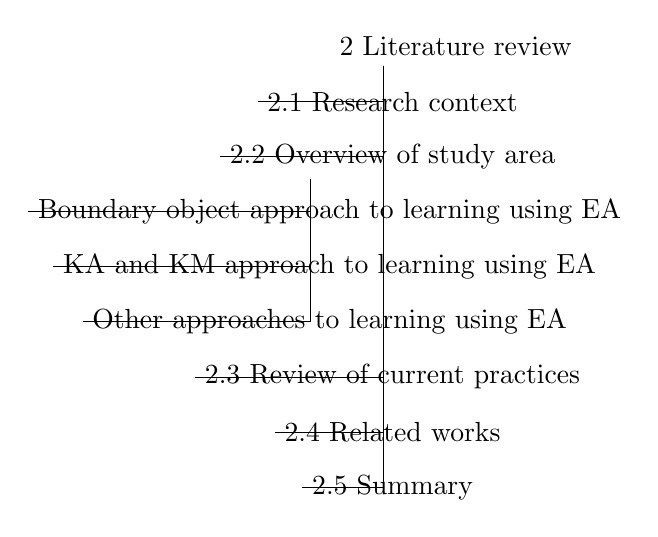
\begin{tikzpicture}[%
  grow via three points={one child at (-0.8,-0.7) and
  two children at (-0.8,-0.7) and (-0.8,-1.4)},
  edge from parent path={(\tikzparentnode.195) |- (\tikzchildnode.west)}]
  \node {2 Literature review}
    child { node {2.1 Research context}}		
    child { node {2.2 Overview of study area} 
        child { node {Boundary object approach to learning using EA}}
        child { node {KA and KM approach to learning using EA}}
        child { node {Other approaches to learning using EA}}
    }
    child [missing] {}				
    child [missing] {}				
    child [missing] {}
    child { node {2.3 Review of current practices}}
    child { node {2.4 Related works}}
    child { node {2.5 Summary}};	
\end{tikzpicture}
    \caption{Structure of Literature review chapter}
    \label{fig:2-TOC}
\end{figure}
 
This section summarises the previous work that cover the same or a similar topic and explores potential research gaps. It also illustrates the current state of the art in smart city \gls{ea}.

The structure of the chapter is shown in figure \ref{fig:2-TOC}.
\section{Research context}

\begin{figure}
    \centering
    %\begin{turn}{-90}
    \makebox[\textwidth][c]{
        \tikzset{
  box/.style={
    draw,
    rectangle,
    minimum height=1cm,
    fill=white,
    align=center,
    inner sep=1ex
  }
}

\begin{tikzpicture}[]
    \iffalse
    \begin{scope}[on background layer]
         \node at (-0.5,-3) [box, minimum width=2.5cm, text width=1.8cm, minimum height=9cm, fill=cyan, align=north] (planning) {Integrated Planning and design};
        \node[box, minimum width=2.5cm, text width=1.8cm, minimum height=9cm, fill=cyan, right= 2mm of planning] (common) {Common energy market};
        \node[box, minimum width=2.5cm, text width=1.8cm, minimum height=9cm, fill=cyan, right= 2mm of common] (community) {Community- xChange};   
    \end{scope}
    \fi
    % Context - Inner
    \node[box, opacity=0.8, text width=\textwidth/2]  (context) {Context};
    \node[box, opacity=0.8, below=2mm of context, text width=\textwidth/2] (service) {Value Added Services};
    \node[box, opacity=0.8, below=2mm of service, text width=\textwidth/2]  (business) {Business (Virtual Enterprise)};
    \node[box, opacity=0.8, below=2mm of business, text width=\textwidth/2]  (application) {Application and Data Processing};
    \node[box, opacity=0.8, below=2mm of application, text width=\textwidth/2]  (+cityxchange) {\textbf{+CityxChange Data Space}};
    \node[box, opacity=0.8, below=2mm of +cityxchange, text width=\textwidth/2]  (technology) {Technologies};
    \node[box, opacity=0.8, below=2mm of technology, text width=\textwidth/2]  (physical) {Physical Infrastructure};

    % Context - Outer
    \begin{scope}[on background layer]
        \node[box, opacity=0.1, inner sep=1ex, fit=(context) (service) (business) (application) (+cityxchange) (technology) (physical)] (main) {};
    \end{scope}

    % Stakeholder perspective  - Inner
    \node[box, minimum height=\textwidth/2, left=of main] (ownership) {\rotatebox{90}{Ownership and access}};
    \node[box, minimum height=\textwidth/2, left=2mm of ownership] (privacy) {\rotatebox{90}{Privacy \& Trust}};
    \node[box, minimum height=\textwidth/2, left=2mm of privacy] (policy) {\rotatebox{90}{Policies \& Regulations}};
    \node[box, minimum height=\textwidth/2, left=2mm of policy] (stakeholder) {\rotatebox{90}{Stakeholders}};

    % Stakeholder perspective  - Outer
    \begin{scope}[on background layer]
        \node[box, inner sep=1ex, fit=(stakeholder) (policy) (privacy) (ownership),  label={Stakeholder perspective}] (stakeholder) {};
    \end{scope} 

    % Data perspective - Inner    
    \node[box, minimum height=\textwidth/2, right=of main] (interoperability) {\rotatebox{90}{interoperability}};
    \node[box, minimum height=\textwidth/2, right=2mm of interoperability] (security) {\rotatebox{90}{Data security, Risk assessment}};
    \node[box, minimum height=\textwidth/2, right=2mm of security] (governance) {\rotatebox{90}{Data Governance}};
    
    % Stakeholder perspective  - Outer
    \begin{scope}[on background layer]
        \node[box, inner sep=1ex, fit=(interoperability) (security) (governance),  label={Data perspective}] (stakeholder) {};
    \end{scope} 

\end{tikzpicture}
    }
    %\end{turn}
    \caption{EAF used in +CityxChange adapted from \cite{cityxchange-d1.2}}
    \label{fig:4-architecture-before}
\end{figure}


This literature review was conducted to better understand the state of \gls{ea} in smart city projects or similar projects and understand the current research gaps related to \gls{ea} as a tool for learning. It was initiated as a result of work related to +CityxChange where researchers found that their \gls{eaf} might be improved by considering how enterprises learn. Their work is in part documented in \cite{cityxchange}. 
The \gls{eaf} shown in figure \ref{fig:4-architecture-before} was proposed in +CityxChange along with the development process shown in figure \ref{fig:4-architecture-development} and will be used in this thesis as a base to be improved in relation to learning. 
The \gls{eaf} was created for representing \glspl{ict ecosystem} involving multiple stakeholders. Their use of \gls{ict ecosystem} builds on \cite{ictecosystem} that describes \glspl{ict ecosystem} as "encompasses the policies, strategies, processes, information, technologies, applications and stakeholders that together make up a technology environment for a country, government or an enterprise. Most importantly, an ICT ecosystem includes people - diverse individuals who create, buy, sell, regulate, manage and use technology." \cite[p.~3]{ictecosystem}. +CityxChange builds on this description "+CityxChange encompasses not only the data, applications and technologies, but also the policies, regulations, processes, and stakeholders that together constitute the larger technology environment for implementing +CityxChange solutions in each of the cities." \cite[p.~117]{10.1007/978-3-030-22482-0_9}.

The horizontal layers in figure \ref{fig:4-architecture-before} can be referred to as the technology stack. It adds upon terminology used in \gls{togaf}. Data is considered to be an important aspect of the \gls{eaf} as many services and stakeholders rely on data in general and open data in particular. Physical infrastructure is important as smart city development projects often involve physical assets such as electrical grids or measurement devices. 
The context layer contains the drivers for the services being developed. These drivers unify the partners involved in the project. 
The vertical layers describe components that go across the horizontal layers and might be connected to several layers simultaneously. These are often values that effect the system as a whole and not individual components. 

\begin{figure}
    \centering
    
% Define block styles
\tikzset{
    decision/.style={diamond, draw, fill=blue!20, text centered, text width = 1.5cm},
    block/.style={rectangle, draw, fill=blue!20, rounded corners, text width = 1.5cm},
    line/.style={draw, -latex},
    textnode/.style={text width=0.5cm}
}

    
\begin{tikzpicture}[]
    % Place nodes
    \node [block] (components) {Identify and describe components in horizontal layers};
    \node [block, right= 0.8cm of components] (relationships) {Identify and describe relationships};
    \node [block, right= 0.8cm of relationships] (perspectives) {Identify stakeholder and data perspectives};
    \node [decision, right= 0.8cm of perspectives] (iscomplete) {Is model complete};
    \node [block, above= 0.8cm of relationships] (iterate) {Iterate to add detail};
    \node [block, right= 0.8cm of iscomplete] (views) {Identify views to visualise};

   
    % Draw edges
    \path [line] (components.east) -- (relationships.west);
    \path [line] (relationships.east) -- (perspectives.west);
    \path [line] (perspectives.east) -- (iscomplete.west);
    \path [line] (iscomplete.north) |- node [right] {no} (iterate.east);
    \path [line] (iterate.west) -| (components.north);
    \path [line] (iscomplete.east) -- node [above] {yes} (views.west);
\end{tikzpicture}


    \caption{Development process of EA models using the +CityxChange EAF, adapted from \cite{cityxchange-d1.2} figure 5.1}
    \label{fig:4-architecture-development}
\end{figure}

\cite{cityxchange} gives some guiding principles on how the \gls{eaf} could be used, but leaves out specifics so as to allow for greater flexibility for \gls{ea} architects. Figure \ref{fig:4-architecture-development} shows the proposed development process.

\begin{figure}
    \centering
    %\begin{turn}{-90}
    \tikzset{
  box/.style={
    draw,
    rectangle,
    fill=white,
    align=center,
  },
  application/.style={draw, rectangle, fill=blue!20},
  api/.style={draw, rectangle split, rectangle split parts=2, rectangle split part fill={green!20,blue!20}},
  repository/.style={draw, cylinder, rotate=90, fill=blue!20},
  connect/.style={draw, -latex},
  realisation/.style={draw, dashed, -latex}
}

\begin{tikzpicture}[]

    % Context - Inner
    \begin{scope}[on background layer]
        \node[box, text width=\textwidth, text height=\textheight/9]  (context) {};
        \node[box, below=1mm of context, text width=\textwidth, text height=\textheight/9] (service) {};
        \node[box, below=1mm of service, text width=\textwidth, text height=\textheight/9]  (business) {};
        \node[box, below=1mm of business, text width=\textwidth, text height=\textheight/9]  (application) {};
        \node[box, below=1mm of application, text width=\textwidth, text height=\textheight/9]  (+cityxchange) {};
        \node[box, below=1mm of +cityxchange, text width=\textwidth, text height=\textheight/9]  (technology) {};
        \node[box, below=1mm of technology, text width=\textwidth, text height=\textheight/9]  (physical) {};
    \end{scope}

    %Layer text
    \node[box, left=-2cm of context, text width=2cm, minimum height=\textheight/9+2.5mm] (cstart) {Context Layer};
    \node[box, left=-2cm of service, text width=2cm, minimum height=\textheight/9+2.5mm] (sstart) {Service Layer};
    \node[box, left=-2cm of business, text width=2cm, minimum height=\textheight/9+2.5mm] (bstart) {Business Layer};
    \node[box, left=-2cm of application, text width=2cm, minimum height=\textheight/9+2.5mm] (astart) {Application and Data Processing Layer};
    \node[box, left=-2cm of +cityxchange, text width=2cm, minimum height=\textheight/9+2.5mm] (dstart) {Data Space Layer};
    \node[box, left=-2cm of technology, text width=2cm, minimum height=\textheight/9+2.5mm] (tstart) {Technologies Layer};
    \node[box, left=-2cm of physical, text width=2cm, minimum height=\textheight/9+2.5mm] (pstart) {Physical Infrastructure Layer};
    
    %Context layer
    \node[box, right=2mm of cstart, text width= 3.2cm] (cindicator) {Indicator for eMaaS uptake};
    \node[box, right=2mm of cindicator, text width= 3.2cm] (ccontibute) {Contribute to uptake of eMaas};
    \node[box, right=2mm of ccontibute, text width= 3.2cm] (cseamless) {Seamless eMobility concept (of TK)};
    
    %service layer
    \node[box, right=2mm of sstart, text width= 3.2cm] (straffic) {Traffic Management};
    \node[box, right=2mm of straffic, text width= 3.2cm] (sservice) {eMaas Service};
    \node[box, right=2mm of sservice, text width= 3.2cm] (sgreen) {Green Mobility Management};
    
    %Business layer
    \node[box, right=2mm of bstart, text width= 2cm] (bpowel) {Powel};
    \node[box, below=2mm of bpowel, text width= 2cm] (babb) {ABB};
    \node[box, right=2mm of bpowel, text width= 2cm] (btk) {TK};
    \node[box, below=2mm of btk, text width= 2cm] (bfourc) {FourC};
    \node[box, right=2mm of btk, text width= 2cm] (batb) {AtB};
    \node[box, below=2mm of batb, text width= 2cm] (biota) {IOTA};
    
    %Application layer
    \node[api, right=2mm of astart] (apay){API \nodepart{two} AtB Payment ?};
    \node[application, right=2mm of apay, text width= 2.8cm] (atraffic) {Total Traffic Control {TTC} Application};
    \node[application, right=2mm of atraffic, text width= 2.8cm] (aapp) {eM App {Android\textbackslash Web}};
    \node[api, right=2mm of aapp] (aiota) {API \nodepart{two} IOTA ?};  
    
    %Data Space Layer
    \node[repository, right=8mm of dstart,  xshift=5mm, label=left:{AtB}] (datb) {};
    \node[repository, below=12mm of datb, label=left:{Flight info}] (dflight) {};
        \node[box, draw, fill=green!20,xshift=0.5cm,yshift=0.1cm] at (dflight.south) {api};
    \node[repository, right=25mm of dstart, xshift=5mm, label=left:{Nabobil}] (dnabobil) {};
    \node[repository, below=12mm of dnabobil, label=left:{ENTUR}] (dentur) {};
        \node[box, draw, fill=green!20,xshift=0.5cm, yshift=0.1cm] at (dentur.south) {api};
    \node[repository, right=42mm of dstart, xshift=5mm, label=left:{Road Datex}] (ddatex) {};
    \node[repository, below=12mm of ddatex, label=left:{ABB DB}] (dabb) {};
        \node[box, draw, fill=green!20,xshift=0.5cm, yshift=0.1cm] at (dabb.south) {api};
    \node[repository, right=59mm of dstart, xshift=5mm, label=left:{TTC}] (dttc) {};
        \node[box, draw, fill=green!20,xshift=0.5cm, yshift=0.1cm] at (dttc.south) {api};
    \node[repository, below=12mm of dttc, label=left:{City Bikes}] (dbikes) {};
        \node[box, draw, fill=green!20,xshift=0.5cm, yshift=0.1cm] at (dbikes.south) {api};
    \node[repository, right=78mm of dstart, xshift=5mm, label=left:{AVIS}] (davis) {};
        \node[box, draw, fill=green!20,xshift=0.5cm, yshift=0.1cm] at (davis.south) {api};
    \node[repository, below=12mm of davis, label=left:{Taxi}] (dtaxi) {};
    \node[repository, right=100mm of dstart, xshift=5mm, label=left:{IOTA}] (diota) {};
    
    
    %Technology Layer
    \node[box, right=2mm of tstart, text width= 2cm] (tradar) {Radars{\color{red}?}};
    \node[box, right=6.4cm of tradar, text width= 2cm] (tiota) {IOTA};
    
    %Physical Infrastructure Layer
    \node[box, right=2mm of pstart, text width= 1.1cm] (pflights) {Flights};
    \node[box, right=2mm of pflights, text width= 1.1cm] (pbuses) {AtB Buses};
    \node[box, right=2mm of pbuses, text width= 1.1cm] (pev) {EVs};
    \node[box, right=2mm of pev, text width= 1.5cm] (pcharging) {EV Charging station};
    \node[box, right=2mm of pcharging, text width= 1.1cm] (pbikes) {City bikes};
    \node[box, right=2mm of pbikes, text width= 1.1cm] (ptaxis) {ptaxis};
    
    %connections from Physical
    \path [connect] (pbikes.north) -- (dbikes.west); %  (2.3,-14.5)
    \path [connect] (pbuses.north) -- (dentur.west);
    \path [realisation] (pev.north) -- (dabb.west);
    \path [connect] (pcharging.north) --(dabb.west);
    \path [connect] (pflights.north) -- (tradar.south);
    \path [connect] (ptaxis.north) -- (dtaxi.west);
    
    %connections from Technologies
    \path [connect] (tradar.north) -- node[right, near start]{{\color{red}?}} (dflight.west);
    \path [connect] (tiota.north) -- (diota.west);
    
    %Connections from Data space layer
    \path [connect] (dnabobil.east) -- (atraffic.south);
    \path [connect] (ddatex.east) -- (atraffic.south);
    \path [connect] (dentur.east) -- (atraffic.south);
    \path [connect] (datb.east) -- node[right, near start]{{\color{red}?}} (apay.south);
    \path [connect] (davis.east) -- (atraffic.south);
    \path [connect] (davis.east) -- (aiota.south);
    \path [connect] (dabb.east) -- (atraffic.south);
    \path [connect] (dbikes.east) -- (atraffic.south);
    \path [connect] (dttc.east) -- (atraffic.south);
    \path [connect] (dflight.east) -- (atraffic.south);
    \path [connect] (dtaxi.east) -- (atraffic.south);
    \path [connect] (diota.east) -- (aiota.south);
    %node[box, draw, fill=green!20,right, near start]{api}
    %Connections from Application layer
    \path [connect] (apay.north) |- node[right, near start]{{\color{red}?}} (2.5,-7) -| (aapp.130);
    \path [connect] (atraffic.60) -- (0.4, -4.5) -| (straffic.south);
    \path [connect] (aapp.north) -- (3.2,-4.5) -| (sservice.south);
    \path [connect] (aiota.north) |- (4.5,-7) -| (aapp.50);
    
    %Connections from Business layer
    
    %Connections from Service layer
    \path [connect] (sgreen.north) -- (cseamless.south);
    
    %Connections from context layer
\end{tikzpicture}

    %\end{turn}
    \caption{Example of EA model created using the +CityxChange architecture, adapted from figure 5.4 in \cite{cityxchange-d1.2}}
    \label{fig:4-architecture-example}
\end{figure}

Figure \ref{fig:4-architecture-example} shows an example \gls{ict ecosystem} or \gls{ea} model made using the +CityxChange \gls{eaf}.
It only shows the horizontal layers of the system being developed and not the stakeholder perspective or data perspective. The \gls{ea} relates to an \gls{emaas} system. It captures a multi stakeholder project with six identified partners involved in development. These are shown in the business layer. It also shows that the services rely heavily on physical infrastructures and data. 
Although the +CityxChange \gls{eaf} in figure \ref{fig:4-architecture-before}, the development process in figure \ref{fig:4-architecture-development} and the resulting \gls{ea} model in figure \ref{fig:4-architecture-example} were not evaluated on learning, it was developed based on literature on \gls{ea} and smart cities and is believed to cover important aspects of smart city development well. 

\section{Overview of study area}
The field of \gls{ea} has matured since the arrival of the Zachman framework \cite{zachman1987framework} widely regarded as the origin of \gls{ea} as a concept. There exist models to evaluate and compare \gls{ea} \cite{10.1007/978-3-642-24511-4_13} as well as a comprehensive industry for creating and maintaining \gls{ea} in organisations \cite{cameron2013analyzing}. 
Learning within organisations has also been covered in research, but not with unified concepts. 

\subsection{Boundary object approach to learning using EA}
In \cite{doi:10.1177/0162243910377624} \glspl{boundary object} are described as "[\glspl{boundary object}] form the boundaries between groups through flexibility and shared structure—they are the stuff of action" \cite[p.~603]{doi:10.1177/0162243910377624} where boundaries refer to shared spaces or objects. The article mentions that the concept was originally made to analyse cooperative work. The \glspl{boundary object} is where communication happens between group or the method used for communication. The article end with explaining that as the \glspl{boundary object} are meant for simplifying analysis, their definition is tied to scope and scale. \glspl{boundary object} are tied to scope as they must be relevant for the context that is being analysed, and they are tied to scale as the objects must be important enough to warrent analysis.
\cite{abraham2015crossing} looked at \gls{ea} models for learning using \gls{boundary object} perspective. \glspl{boundary object} might be documentation such as \gls{ea} that contain information and can be interpreted differently by individuals based on their background or occupation within an organisation.
\begin{figure}
    \centering

    
% Define block styles
\tikzset{
    property/.style={rectangle, draw, fill=blue!20, text centered, text width = 3cm},
    capacity/.style={rectangle, draw, fill=blue!20, rounded corners, text width = 4cm},
    line/.style={draw, -triangle 90},
    textnode/.style={text width=0.5cm},
}

    
\begin{tikzpicture}[]

    \node [property] (participation) {Participation};
    \node [property, above= 0.5cm of participation] (malleability) {Malleability};
    \node [property, below= 0.5cm of participation] (uptodateness) {Up-to-dateness};
    
    \node [capacity, right= 2cm of participation] (pragmatic) {Pragmatic capacity};
    \node [capacity, below= 2cm of pragmatic] (semantic) {Semantic capacity};
    
    \node [property, left= 2cm of semantic] (annotation) {Annotation};
    \node [property, below= 0.5cm of annotation] (visualization) {Visualization};
    
    \node [capacity, below= 3cm of semantic] (syntactic) {Syntactic capacity};
    
    \node [property, left= 2cm of syntactic] (concreteness) {Concreteness};
    \node [property, above= 0.5cm of concreteness] (accessibility) {Accessibility};
    \node [property, below= 0.5cm of concreteness] (modularity) {Modularity};
    \node [property, below= 0.5cm of modularity] (sharedsyntax) {Shared syntax};

    % Draw edges
    \path [line] (participation.east) -- (pragmatic.west);
    \path [line] (malleability.east) -- (pragmatic.north west);
    \path [line, loosely dashed] (uptodateness.east) -- (pragmatic.south west);
    
    \path [line] (annotation.east) -- (semantic.west);
    \path [line] (visualization.east) -- (semantic.south west);
    
    \path [line] (concreteness.east) -- (syntactic.west);
    \path [line, loosely dashed] (accessibility.east) -- (syntactic.north west);
    \path [line] (modularity.east) -- (syntactic.west);
    \path [line] (sharedsyntax.east) -- (syntactic.south west);
    
    \path[line] (semantic.north) -- (pragmatic.south);
    \path[line] (syntactic.north) -- (semantic.south);

\end{tikzpicture}



    \caption{Knowledge boundary properties and how they affect capacity. Adapted from \cite{abraham2015crossing}}
    \label{fig:knowledge-boundary-properties}
\end{figure}

The research aims to find the properties of \gls{ea} models that enable syntactic, semantic or pragmatic capacity for \glspl{boundary object}. knowledge is transferred between groups or individuals using \glspl{boundary object} and knowledge is translated. Its literature review found 11 boundary object properties;  modularity, Abstraction, concreteness, shared syntax, malleability, visualization, annotation, versioning, accessibility, up-to-dateness, stability and participation. They hypothesised that accessibility, concreteness, modularity and shared syntax increase syntactic capacity of \glspl{boundary object}. while annotation and visualization increase semantic capacity and malleability, participation and up-to-dateness increase pragmatic capacity. syntactic capacity increases semantic capacity which in turn increase pragmatic capacity. Their theory is that for the ability to learn one needs the capacity of \glspl{boundary object} and capabilities. Figure \ref{fig:knowledge-boundary-properties} shows the relationship between properties and capacities. The findings did not support the hypothesis of causation from availability and up-to-dateness to syntactic capacity, but postulate  that it is a requirement for learning. The conclusion is that \glspl{boundary object} should be connected to the domain concretely and that the visualisation should be efficient to enhance learning. 
\begin{table}
    \centering
    
    \begin{tabular}{|l|p{\textwidth/2}|}
        \hline
        Property & short Explanation \\ \hline
        Malleability & Supports changes by all communities using the \gls{boundary object}.  \\ \hline
        Participation & The relevant communities participate in the creation and maintenance of the \gls{boundary object}.  \\ \hline
        Up-to-dateness & The \gls{boundary object} is updated and communities are informed. \\ \hline
        Annotation & Individual communities can add additional information for local use.  \\ \hline
        Visualization & The \gls{boundary object} has a physical representation. \\ \hline
        Accessibility & The \gls{boundary object} is known about and accessible to the communities. \\ \hline
        Concreteness & The \gls{boundary object} contains information relevant for the specific communities. \\ \hline
        Modularity & Parts of the \gls{boundary object} can be viewed in seclusion from the rest while maintaining correctness. \\ \hline
        Shared syntax & A common understanding exist for interpretation of the \gls{boundary object}.  \\ 
        \hline
    \end{tabular}
    \caption{A short explanation of Boundary object properties from \cite{abraham2015crossing}}
    \label{tab:2-boundary-properties}
\end{table}




Table \ref{tab:2-boundary-properties} shows a short explanation of the properties.

\subsection{KA and KM approach to learning using EA}
\cite{10.1371/journal.pone.0127005} looks at \gls{ea} through the lens of \gls{ka} and \gls{km} specifically within large scale organisations. They note that \gls{ea} changed from a classic perspective, focusing on domain specific systems to large-scale architecting with focus on abstract, meta-level systems with more intensive communication infrastructures. This shift required more complex architectures. \gls{ka} is formed by knowledge reservoirs and knowledge flows and is seen as a component of enterprise assets similarly to \glspl{boundary object}. The research views \gls{ka} as "incorporates the manner of creating knowledge, its application and learning within enterprises."\cite[p.~4]{10.1371/journal.pone.0127005} The elements of \gls{ka} are people, processes, behaviours, technology and content. They conducted a literature review on \gls{ka} and found that \gls{ka} did not sufficiently address large-scale architecting, did not have suitable methodology and did not have a supervising framework. The research proposes a \gls{ka} methodology and framework to alleviate these problems. They base their \gls{ka} framework on zachman's \gls{eaf} as it is seen as an accepted standard that is both malleable formal and robust. In their framework the focus is on the planner perspective, owner perspective and designer perspective, while the other perspectives are seem as outside the scope of \gls{ka}. Their methodology is based on CommonKADS, a methodology commonly used for engineering in \gls{km} where the goal of \gls{km} is to create  models for knowledge recounting that can either be in the context category, concept category or artefact category. The researchers used "leadership, culture and structure, processes, explicit knowledge, implicit knowledge, knowledge hubs and centers, market leverage, measures, personnel skills and technological infrastructure"\cite[p.~17]{10.1371/journal.pone.0127005} as the metrics to evaluate their framework.

\subsection{Other approaches to learning using EA}
\cite{narman2016using} conducted a literature review on theoretical approaches for creating and evaluating organisational structures impact on motivation and learning. They found that most approaches were insufficient for an evaluation framework and advocated for theories with a holistic approach to organisation modelling. They selected Mintzberg \cite{mintzberg1979structuring} for their research. They used it with \gls{uml} and \gls{ocl} to create an evaluation model. 

\section{Review of current practices}
The use of \gls{ict} architecture and \gls{ea} in smart cities varies greatly. There is currently no best practices for determining what \gls{ea} to use or \gls{ict} architecture patterns to use.
\cite{kakarontzas2014} looked at important properties of smart cities that would be architecturally significant and important for deciding \gls{ict} infrastructure. It also looked at the current business aspects of the \gls{it} support infrastructure. It conducted a questionnaire comprising of questions regarding architecture, data sources, management, funding and project objectives. It found that organisational structure, business processes, information systems and infrastructure were the most important dimensions for \gls{ea}. The research conclude that the \gls{ict} architecture should be generic with a focus on interoperability and that performance was not a critical concern. They suggest the \gls{ict} architecture to use a layered architecture and \gls{mvc} pattern with \gls{api} facade and messaging architecture.
However \cite{7580810} concluded from their research that no \gls{ict} architecture would be generalizable enough to benefit new smart city projects. They ascertain that \gls{adm} is a good approach to smart city development and that smart cities can be viewed as enterprises. This is supported by \cite{pourzolfaghar2016types} which focused on the business aspect of \gls{ea}. They found that the abstract architectures proposed did not fulfil the business requirements and also recommend \gls{adm}. \cite{7580810} separated the \gls{adm} into three parts; Why, what and how, then looked at how the literature related to those separations. \gls{adm} was found to sufficiently cover the smart city issues in the literature. The issues discussed in the paper did not cover learning or knowledge transfer, so it is uncertain if \gls{adm} would be sufficient when focused on learning.

\section{Related work}
\setlength\LTleft{-3.3cm}
\setlength\LTright{+3.3cm}
\begin{longtable}{
    |p{\textheight/7}|p{\textheight/8}|p{\textheight/10}|p{\textheight/8}|
     p{\textheight/3}|
}
    \hline
    Authors & article & Purpose & context and categorisation & Model \\ \hline
        
    Kakarontzas, George - Anthopoulos, Leonidas - Chatzakou, Despoina -Vakali, Athena
    & A Conceptual Enterprise Architecture Framework for Smart Cities - A Survey Based Approach 
    & Propose generic \gls{ict} architecture 
    & \begin{itemize}[leftmargin=0.3cm]
        \item Context: EADIC - (Developing an Enterprise Architecture for Digital Cities)
        \item Categories: \gls{ict} architecture and Smart Cities
    \end{itemize} 
    & ICT architecture: host organisation of an application has a \gls{ui} \gls{mvc} layer with synchronous \gls{api} calls to Business logic layer that communicates with local data storage and \gls{mom} server.  The \gls{mom} server talks to otter applications and integrates with the municipality. The \gls{ui} is accessed by a browser. 
    \\ \hline     
     
    Hämäläinen, Mervi
    & A Framework for a Smart City Design: Digital Transformation in the Helsinki Smart City
    & "Shed light on the elements that are relevant for robust digital transformation" \cite[p.~65]{hamalainen2020framework} by presenting a design framework
    & \begin{itemize}[leftmargin=0.3cm]
        \item Context: Helsinki Smart City
        \item Categories: Smart Cities and Design framework
    \end{itemize} 
    & Evaluation framework: 11 values that have values from 0 to 3. The 11 include four dimensions; Smart city strategy, Technology - Digital technologies, Governance - orchestration and Stakeholders, and 7 sub-values; capabilities, data, technology experimentation, security and privacy, vertical and horizontal scope, funding and metrics, and stakeholder values. 

    \\ \hline
     
    Abraham, Ralf - Aier, Stephan - Winter, Robert
    & Crossing the line: overcoming knowledge boundaries in enterprise transformation 
    &  Understanding properties of \gls{ea} that allow shared understanding during enterprise transformations
    & \begin{itemize}[leftmargin=0.3cm]
        \item Context: Enterprise transformation research
        \item Categories: \gls{ea}, Knowledge boundaries and Enterprise transformation
    \end{itemize} 
    & See \ref{fig:knowledge-boundary-properties}
    \\ \hline
     
    Mamkaitis, Aleksas - Bezbradica, Marija -Helfert, Markus 
    & Urban Enterprise: a review of Smart City frameworks from an Enterprise Architecture perspective 
    & Understand EA in smart cities 
    & \begin{itemize}[leftmargin=0.3cm]
        \item Context: Smart city research
        \item Categories: Smart Cities, \gls{ea} and \gls{togaf}
    \end{itemize}  
    & Suggests using \gls{adm}
    \\ \hline
     
    Pourzolfaghar, Zohreh - Bezbradica, Marija - Helfert, Markus 
    & Types of IT architectures in smart cities–a review from a business model and enterprise architecture perspective 
    & Evaluate architectures based on business perspective 
    & \begin{itemize}[leftmargin=0.3cm]
        \item Context: \gls{ea} business Layer research
        \item Categories: \gls{ea}, Business perspective and Smart city
    \end{itemize}  
    & Suggests using \gls{adm}
    \\ \hline
     
    Varaee, Touraj  - Habibi, Jafar - Mohaghar, Ali 
    & Presenting an Approach for Conducting Knowledge Architecture within Large-Scale Organizations 
    & Finding a valid methodology and framework for \gls{ka} within large scale organisations.
    & \begin{itemize}[leftmargin=0.3cm]
        \item Context: Large scale organisations research
        \item Categories: \gls{ea}, Knowledge and \gls{ka}
    \end{itemize}
    & \gls{ka} framework: Rectangular cuboid  (7 by 6 by 6) based on zachman
    \\ \hline
     
    L. LouwI, - H.E. EssmannII - N.D. du PreezI - C.S.L. Schutte 
    & Architecting the enterprise towards enhanced innovation capability 
    & Proposing a \gls{eaf} to support innovation
    & \begin{itemize}[leftmargin=0.3cm]
        \item Context: Enterprise research
        \item Categories: \gls{ea} and Innovation capabilities 
    \end{itemize}
    & \gls{eaf}: consisiting of strateguc intent, value chain and process, information, human resources, physical assets, organisational, performance, financial and governance architecture. It is viewed as influenced by suppliers partners customers and external influences.
    \\ \hline
     
    Närman, Pia -  Johnson, Pontus - Gingnell, Liv 
    & Using enterprise architecture to analyse how organisational structure impact motivationand learning 
    & Proposing an evaluation framework of motivation and learning based on \gls{ea} 
    & \begin{itemize}[leftmargin=0.3cm]
        \item Context: Organisational structures research
        \item Categories: \gls{ea}, motivation and learning
    \end{itemize}  
    & Evaluation model: based on \gls{uml} and \gls{ocl}
    \\ \hline
     
    \caption{Related work relevant for this thesis}
    \label{tab:related-works}
\end{longtable}

\setlength\LTleft{0cm}
\setlength\LTright{0cm}

\iffalse % Summaries if those are relevant
%A Conceptual Enterprise Architecture Framework for Smart Cities - A Survey Based Approach
& Aims to find important properties of smart cities and propose an appropriate \gls{ict} architecture. It also aims to understand the current business aspects of the \gls{it} support infrastructure. A questionnaire was used and found organisational structure, business processes, information systems and infrastructure to be most important. Suggests a generic infrastructure with a focus on interoperability. 

%A Framework for a Smart City Design: Digital Transformation in the Helsinki Smart City
& Presents smart city projects as digital transformation that changes the capabilities and organisational structure of the organisation (city) and need consideration of long term effects. The projects should allow the city to continuously evolve with long term goals. It stresses that it is a complex system and advocates for open data where possible. It found that quadruple helix collaboration had fostered technology acceptance in the city. An evaluation framework is presented
\fi


Some of the related literature used in this paper is summarised in table \ref{tab:related-works}. 

\section{summary}
There is substantial research on smart city and how it relates to \gls{ea}, but little is documented on how cities learn from \gls{ea}.
\chapter{Methodology}
\label{chap:methodology}

This section covers the approach taken to answer the research questions and the different research methods used in this work to ensure quality.
\section{Research methodology}
\subsection{Research flow}
\begin{figure}
    \centering
    \rotatebox{-90}{
        %\missingfigure{Make diagram show research flow}
% Define block styles
\tikzset{
    objective/.style={rectangle, draw, fill=blue!20, rounded corners, text width=\textheight/4.5},
    method/.style={rectangle, draw, fill=green!20, text width=\textwidth/4.5},
    action/.style={rectangle, draw, fill=blue!20, text width=\textwidth/4.5},
    gap/.style={rectangle, draw, fill=red!20, rounded corners, text width=\textwidth/4.5},
    section/.style={rectangle, draw, fill=yellow!20, text width=\textwidth/4.5},
    line/.style={draw, -latex},
    box/.style={rectangle, draw, fill=white, align=center, text height=0.9\textwidth}
}

    
\begin{tikzpicture}[]
    
    % research gaps and problems
    \node[gap] at (-0.5,4) (citylearning) {Limited literature on how to learn from smart city projects and initiatives};
    \node[gap, below=1cm of citylearning] (ealearning) {Limited literature on how useful \gls{ea} is for learning};
    \node[gap, below=3.5cm of ealearning] (eaf+city) {The \gls{eaf} proposed in +CityxChange does not focus on learning};
    
    % Research objectives
    \node[objective] at (5.2,4) (ro1) {RO1: Gain a better understanding of how the current state of \gls{ea} facilitates learning and how the proposed smart city \gls{eaf} diverge.};
    \node[objective, below=0.3cm of ro1] (ro2) {RO2: Understand which aspects of \gls{ea} is perceived to be of use and enhance learning in smart city projects.};
    \node[objective, below=0.3cm of ro2] (ro3) {RO3:Understand how \gls{ea} can transfer and retain knowledge within an organisation and shared with other organisations.};
    \node[objective, below=0.3cm of ro3] (ro4) {RO4:Provide recommendations for improvement to the \gls{eaf} used in +CityxChange.};
    
    % Research methods
    \node[method] at (10,5.5) (literaturereview) {Literature review};
    \node[method, below= 4cm of literaturereview] (survey) {Survey method};
    \node[method, below= 3cm of survey] (model) {Model proposition};
    \node[method, below= 0.5 of model] (expert) {Expert evaluation};

    %Research actions
    \node[action, below= 0.5cm of literaturereview] (initliterature) {Initial literature review};
    \node[action, below= 0.5cm of initliterature] (literature) {Continued literature review};
    \node[action, below= 0.5cm of survey] (questionnaire) {Questionnaire with individuals working on +CityxChange};
    \node[action, below=0.5 of expert] (interview) {Interview};
    
    %Documented by
    % \node[section] at (15.3,3.7) (secliterature) {Chap1: Introduction};
    \node[section] at (15.3,3.7) (secliterature) {Chap2: Literature review};
    % \node[section, below= 2.8cm of secliterature] (secmethod) {Chap3: Methodology};
    \node[section, below= 1.5cm of secliterature] (secgathering) {Chap4: Gathering data from +CityxChange};
    % \node[section, below= 2.8cm of secliterature] (seccxcevaluation) {Chap5: +CityxChange EAF evaluation};
    \node[section, below= 2.5cm of secgathering] (secmodel) {Chap6: Proposed model};
    \node[section, below= 0.3cm of secmodel] (secevaluation) {Chap7: Model evaluation};
    \node[section, below= 0.2cm of secevaluation] (secresult) {Chap8: Results and discussion};
    % \node[section, below= 2.8cm of secliterature] (secmodel) {Chap6: Proposed model};
    
    % Draw connections);
    \path [line] (initliterature.10) -|  (12,6.5) -- node [near end, above] (informliterature) {Informs} (-2.7,6.5) |- (citylearning.west);
    \path [line] (initliterature.10) -|  (12,6.5) -- (-2.7,6.5) |- (ealearning.west);
    
    \path [line] (citylearning.east) -- node [midway, above, sloped] {led to} (ro1.west);
    \path [line] (citylearning.east) -- (ro2.west);
    \path [line] (ealearning.east) -- (ro1.west);
    \path [line] (ealearning.east) -- (ro2.west);
    \path [line] (ealearning.east) --  node [midway, above] {led to} (ro3.west);
    \path [line] (ealearning.east) -- (ro3.west);
    \path [line] (eaf+city.east) -- node [midway, above, sloped] {led to} (ro4.west);
    
    \path [line] (ro1.east) -- (initliterature.west);
    \path [line] (ro1.east) -- (literature.west);
    \path [line] (ro2.east) -- (literature.west);
    \path [line] (ro2.east) -- (survey.west);
    \path [line] (ro3.east) -- (literature.west);
    \path [line] (ro3.east) -- (survey.west);
    \path [line] (ro4.east) -- (model.west);
    
    \path[line] (survey.south) -- node [midway, right] {Using} (questionnaire.north);
    \path[line] (literaturereview.south) -- node [midway, right] {With} (initliterature.north);
    \path[line] (initliterature.south) -- node [midway, right] {Followed by} (literature.north);
    \path[line] (initliterature.east) -- node [midway, above] {reported in} (secliterature.west);
    \path[line] (literature.east) -- (secliterature.west);
    \path[line] (survey.east) -- node [midway, above] {reported in} (secgathering.west);
    \path[line] (model.south) -- node [midway, right] {Evaluated with} (expert.north);
    \path[line] (model.east) -- node [midway, above, sloped] {reported in} (secmodel.west);
    \path[line] (expert.south) -- node [midway, right] {Using} (interview.north);
    \path[line] (expert.east) -- node [midway, above, sloped] {reported in} (secevaluation.west);
    
    \path[line] (secliterature.east) -- (17.3,3.7) |- (secresult.east);
    \path[line] (secgathering.east) -- (17.3,0.9) |- (secresult.east);
    \path[line] (secmodel.east) -- (17.3,-2.9) |- (secresult.east);
    \path[line] (secevaluation.east) -- (17.3,-4.2) |- (secresult.east);
    
    % Lanes
    \begin{scope}[on background layer]
        \node[box, text width=\textheight/4.5, 
            label={Gaps in the literature}]  (existingliterature) {};
        \node[box, right=1mm of existingliterature, text width=\textheight/4.2, 
            label={Research objectives}] (objectives) {};
        \node[box, right=1mm of objectives, text width=\textheight/4.9,
            label={Research process}]  (methods) {};
        \node[box, right=1mm of methods, text width=\textheight/5,
        label={Thesis structure}]  (documented) {};
    \end{scope}
    
    % Diagram explanation
    \node[gap, above= of existingliterature] (explaingap) {<Gap in the literature/problem>};
    \node[objective, right=2mm of explaingap] (explainobjective) {<Research objective>};
    \node[method, right=2mm of explainobjective] (explainmethod) {<Research method>};
    \node[action, right=2mm of explainmethod] (explainaction) {<Research activity>};
    \node[section, right=2mm of explainaction] (explainsection){<Thesis section/chapter>};
    
\end{tikzpicture}

    }
    \caption{How research was conducted and documented in this thesis.}
    \label{fig:3-research-flow}
\end{figure}

Figure \ref{fig:3-research-flow} shows a visualisation of how the identified problems in the literature motivated the research objectives, how the objectives were reached through the research process and how the thesis documents the process and results.

The research started with an initial literature review in order to identify gaps or problems in the literature. The results of the review informed the research objectives. 
The literature review was continued after the objectives were identified and progressed alongside with the other research activities. The other research activities that were done was a survey, model proposition and expert evaluation. The survey was conducted to better understand the use of \gls{ea} in a smart city project context, how the +CityxChange \gls{eaf} in particular contributed to the project and how it and \gls{ea} in general related to +CityxChange's learning efforts.
The survey was implemented using an online questionnaire.
The data gathered from the survey was used with the data from the literature review in order to identify the requirements and to propose a model consisting of an \gls{eaf}, a development process and \gls{ea} elements. An \gls{ea} element is considered as a visual representation of an uninstantiated entity that can be used in an \gls{ea} model. When the element is instantiated it becomes a component. 
The model was evaluated with an expert evaluation, using semi-structured interviews. 

\subsection{Literature Review approach}
\begin{table}
    \centering
    \begin{tabular}{|c|p{0.8\textwidth}|}
        \hline
        ID & Question \\ \hline
        Q01 & Is the research aim clearly stated? \\ \hline
        Q02 & Is the research method clearly stated?\\ \hline
        Q03 & Is the research context clear? \\ \hline
        Q04 & Is the research grounded in theory?\\ \hline
        Q05 & are the results clearly presented?\\ \hline
        Q06 & Is validity of research discussed?\\ \hline
        Q07 & Does it discuss use of Enterprise architecture?\\ \hline
        Q08 & Does it discuss knowledge management, innovation, knowledge transfer or learning without artificial intelligence or machine learning?\\ \hline
        Q09 & Does it discuss smart city, smart city services or construction planning?\\ \hline
        Q10 & Uses a technology acceptance model or similar.\\ \hline
    \end{tabular}
    \caption{Literature screening questions and relevance questions.}
    \label{tab:sceeningQuestions}
\end{table}
\iffalse
\begin{figure}
    \centering
    \iffalse
% Define block styles
\tikzset{
    source/.style={rectangle split, split parts=2, draw, fill=blue!20, rounded corners, text width=\textheight/4.5},
    identified/.style={rectangle split, split parts=2, draw, fill=blue!20, rounded corners, text width=\textheight/4.5},
    screening/.style={diamond, draw, fill=blue!20, text centered, text width = 1.5cm},
    selected/.style={rectangle split, split parts=2, draw, fill=green!20, text width=\textwidth/4.5},
    exclusion/.style={rectangle, draw, fill=red!20, rounded corners, text width=\textwidth/4.5},
    section/.style={rectangle, draw, fill=yellow!20, text width=\textwidth/4.5},
    line/.style={draw, -latex},
}

    
\begin{tikzpicture}[]
    % Queries
    \node[Source] () {
        \nodepart{one}
            Query
        \nodepart{two}
             "Knowledge transfer"  AND "Enterprise Architecture"
    }
    \node[Source] () {
        \nodepart{one}
            Query
        \nodepart{two}
            "Enterprise Architecture" AND "smart cities"
    }
    \node[Source] () {
        \nodepart{one}
            Query
        \nodepart{two}
            cities as learning innovation ecosystems
    }
    \node[Source] () {
        \nodepart{one}
            Query
        \nodepart{two}
            knowledge transfer across cities
    }
    \node[Source] () {
        \nodepart{one}
            Query
        \nodepart{two}
            Learning from "Enterprise Architecture models"
    }
    
    % Other sources
    \node[Source] () {
        \nodepart{one}
            Mentioned
        \nodepart{two}
            From author
    }
    \node[Source] () {
        \nodepart{one}
            Mentioned
        \nodepart{two}
            From reference
    }
    \node[Source] () {
        \nodepart{one}
            Mentioned
        \nodepart{two}
            From supervisor
    }
    
    % Identified
    \node[identified] () {
        \begin{itemize}[leftmargin=0.3cm]
            \item total selected (n=89)
        \end{itemize}
    }
    
    % Screening
    \node[screening] () {Screening}
    
    %Exclusion 
    \node[exclusion, right of screening] {Rejected (n=18)}
    
    %Pending
    
\end{tikzpicture}
\fi
    \caption{Inclusion and exclusion of literature}
    \label{fig:screening}
\end{figure}
 \fi
\begin{itemize}
    \item \textbf{Query construction:} Literature was queried using the search engines at google scholar, web of science, Scopus and Oria. The search terms used included: "Enterprise Architecture" AND "smart cities", Learning from "Enterprise Architecture models", cities as learning innovation ecosystems, and knowledge transfer across cities. Additional literature was gathered based on references and authors.
    
    \item \textbf{Screening:} Relevance and quality was assessed to exclude articles given by the query. The questions used to assess quality and relevance are listed in table \ref{tab:sceeningQuestions}. \iffalse and the result of the query and screening is displayed in figure \ref{fig:screening}. \fi
    
\end{itemize}

\subsection{Survey approach}
\begin{itemize}
    \item \textbf{Data collection method:} A questionnaire was used to gather data. The questions were based on the initial literature review discussed in chapter \ref{chap:literature} and based on the \gls{tam} to indicate potential of the \gls{eaf} proposed in +CityxChange.
    The questionnaire was made primarily for this thesis, but also to be used for a delivery within +CityxChange project \cite{cityxchange-d1.2}. As a result not all questions of the questionnaire were deemed relevant for this thesis. The questionnaire consisted of 6 parts; information about the questionnaire and consent to use and publish data, demographic on participants, view of \gls{ea} in general, view of \gls{eaf} used in +CityxChange, view of how \gls{ea} in general and the \gls{eaf} in particular relates to knowledge transfer and a final section for free-text answers with the opportunity to give feedback that the participants felt were missing or required clarification.
    In total there were 47 questions and the questions were given via nettskjema.no due to an existing data processing agreement with \gls{ntnu}. Permission to process personal data was granted by the \gls{nsd} and all participant consented to the use of relevant data.
    \item \textbf{Population/sampling:}
    The questionnaire was given online to 42 participants with a connection to +CityxChange. The criteria for receiving the questionnaire was a familiarity with the \gls{eaf} used in +CityxChange. Of the 42 asked participants 13 participated. A question within the questionnaire asked for their familiarity with the \gls{eaf} on which one participant indicated that they were not familiar with the \gls{eaf}. Although this indicate that this person did not fit the criteria for receiving and answering the questionnaire, the answers were still included in the analysis. 
    \item \textbf{Data analysis:} Due to the limited number of answers, a qualitative approach were used for most questions including all free-text questions. Percentages and graphics were calculated and created by nettskjema. 
    \iffalse Analysis was conducted using \gls{spss}. \fi
\end{itemize}

\subsection{Model proposition approach}    
The model proposition followed a designed and creation process with five steps
\begin{itemize}
    \item \textbf{Awareness:} The needs of the model were gathered through the literature review and questionnaire.
    \item \textbf{Suggestion:} A potential solution to the needs were suggested.
    \item \textbf{Development:} A model implementing the suggestions were developed.
    \item \textbf{Evaluation:} The model was evaluated with expert evaluation
    \item \textbf{Conclusion:} The results were analysed and reported in this thesis.
\end{itemize}

\subsection{Expert evaluation approach}
{\centering
\begin{longtable}{|p{2.3cm}|p{4.5cm}|p{5cm}|}
    \hline
        Themes & Questions & Motivation\\ \hline
        \multirow{1}{2.3cm}{Role of \gls{ea}} 
            & \multirow{2}{4.5cm}{First off, I would like to know a bit about how you view \gls{ea} as a whole. So, What do you consider to be the job of \gls{ea}?} & Lead off with a question the participant is likely to already have an opinion on. \\ \cline{3-3}
            & & Understand whether or not the proposed model is aligned with the needs of the participant. \\
        \hline
        \multirow{3}{2.3cm}{Participation,  Malleability, annotation and shared syntax} 
            & \multirow{2}{4.5cm}{Who do you think has a use for the \gls{ea} models?} & Understand the usage context. \\ \cline{3-3}
            & & Understand if the \gls{eaf} is aligned with the users needs. \\ \cline{2-3}
            & \multirow{1}{4.5cm}{Do you think the suggested \gls{eaf} allow them (groups of users) to adequate model their perspective of the \gls{ea}? (Why, why not?)} & Understand if it supports the different usage contexts \\ \cline{3-3}
            & & Understand if there are perspectives with misssing elements. \\ \cline{2-3}
            & \multirow{2}{4.5cm}{Do you think that any part of the \gls{eaf} could be interpreted differently by some of the users? (Why, why not?)} & Understand if the users would have a common understanding of the resulting model. \\ \cline{3-3}
            & & Understand if the syntax or terminology has contradictory meanings within between different communities. \\
        \hline
        \multirow{2}{2.3cm}{Visualization, Accessibility} 
            & \multirow{1}{4.5cm}{Do you think the \gls{eaf} would give an efficient representation of the \gls{ea}? (why, why not)} & Understand whether or not the visualization is easy to interpret and important components can quickly be identified. \\ \cline{2-3}
            & \multirow{1}{4.5cm}{Do you think the \gls{eaf} will be understood by non-practitioners of \gls{ea}? (why, why not)} & Understand if the complexity is too high or if it creates problems when using the model to introduce the \gls{ea} to new personnel. \\
        \hline
        \multirow{2}{2.3cm}{+CityxChange, concreteness} 
            & \multirow{1}{4.5cm}{Do you think the \gls{eaf} is adequate for +CityxChange projects? (why, why not)} & Understand if the needs of +CityxChange is aligned with the \gls{eaf}. \\ \cline{2-3}
            & \multirow{1}{4.5cm}{Is there anything you think is unnecessary in the \gls{eaf}? (why, why not)} & Understand whether or not the \gls{eaf} is to broad or can be simplified without negative effects. \\
        \hline
        \multirow{1}{2.3cm}{Modularity} 
            & \multirow{2}{4.5cm}{Would the \gls{eaf} allow specific problems to be viewed separately from the entire \gls{ea} while maintaining correctness or validity? (why, why not) } & Understand if the \gls{eaf} supports modularity. \\ \cline{3-3}
            & & Understand if the different users of the model can work on what is relevant to them without unnecessary interference. \\
        \hline
        \multirow{3}{2.3cm}{Technology acceptance} 
            & \multirow{1}{4.5cm}{Do you think the \gls{eaf} would be usefull for +CityxChange or smart city development?} & Understand "perceived usefulness" as it relates to \gls{tam} and +CityxChange and the smart city development projects. \\ \cline{2-3}
            & \multirow{1}{4.5cm}{Do you think the \gls{eaf} would be easy to use?} & Understand "perceived ease of use" as it relates to \gls{tam}. \\ \cline{2-3}
            & \multirow{1}{4.5cm}{Would you use this yourself or recommend it to others?} & Understand "intent to use" as it relates to \gls{tam}. \\
    \hline
    
    \caption{Interview questions for expert evaluation of proposed EAF}
    \label{tab:4-evaluation-interview}
\end{longtable}}
\begin{itemize}
    \item \textbf{Data collection method:} A semi structured interview was used for the evaluation. The interview consisted of six themes; "Role of \gls{ea}", "Participation,  Malleability, annotation and shared syntax", "Visualization, Accessibility", "+CityxChange, concreteness", "Modularity", "Technology acceptance". The themes and relevant questions are listed in table \ref{tab:4-evaluation-interview}. The themes are based on the \gls{boundary object} discussed in \cite{abraham2015crossing} and \gls{tam}. 12 questions were prepared before the interview and used to guide the interview. 30 minutes were allocated to each interview as the participants were busy and requested that it be kept short. Not all questions were asked during every interview due to the time constraint and nature of semi structured interviews. The themes were still covered. The interviewees were given a short introduction to the proposed model consisting of the proposed \gls{eaf}, development process and \gls{ea} elements, but were not given definitions of the layers or use case for the elements, unless explicitly requested. This was done to determine if the terminology used was appropriate and intuitive. Intuitiveness was one of the problems identified through the questionnaire and seen as important for the evaluation.
    \item \textbf{Population/sampling:} Three participants were selected and interviewed separately. All three were selected based on their knowledge of either the +CityxChange \gls{eaf} or learning within smart city projects.
    The qualities of the participants that were important for the sampling process were: 
    \begin{itemize}
        \item Participant 1: Experienced with \gls{ea} and one of the architects behind the \gls{eaf} used in +CityxChange.
        \item Participant 2: Familiar with \gls{ea} for smart cities and a contributor to the \gls{eaf} used in +CityxChange.
        \item Participant 3: Not familiar with \gls{ea}, but experienced with urban planning and learning across cities. 
    \end{itemize}
\end{itemize}
\chapter{Gathering data from +CityxChange} 
\label{chap:survey}

This section introduces a survey conducted to understand the the needs of the +CityxChange \gls{eaf}.

\section{Motivation behind the survey}
A survey was found to be the best approach to understanding the role of \gls{ea} in smart city projects and how it relates to learning. +CityxChange was chosen as a project where the survey could be undertaken. As an ongoing lighthouse project involving two lighthouse cities and five follower cities, it is believed to be representative of smart city projects.
The main motivation of the survey was to gain insights from the +CityxChange employees that had used the +CityxChange \gls{eaf}. Their understanding could be used to improve \gls{ea} in regards to learning in smart city projects. The survey was made to understand the context where the \gls{ea} was used, who were using it, what their attitudes towards it were and what could be done to improve it. The secondary motivation was for this information to be used to improve the +CityxChange \gls{eaf} to support learning across cities.
The full questionnaire can be found in apendix \ref{app:questionnaire}.

\section{Survey Results}
\subsection{Demographic}
The demographics section asked for gender, age represented organisation and role within organisation.
Overall the demographic information is inline with what was expected in the field of \gls{ea} and computer science. 
The roles reported varied, but could be summed up as researchers, developers, engineers and managerial roles.
\begin{figure}
    \centering
    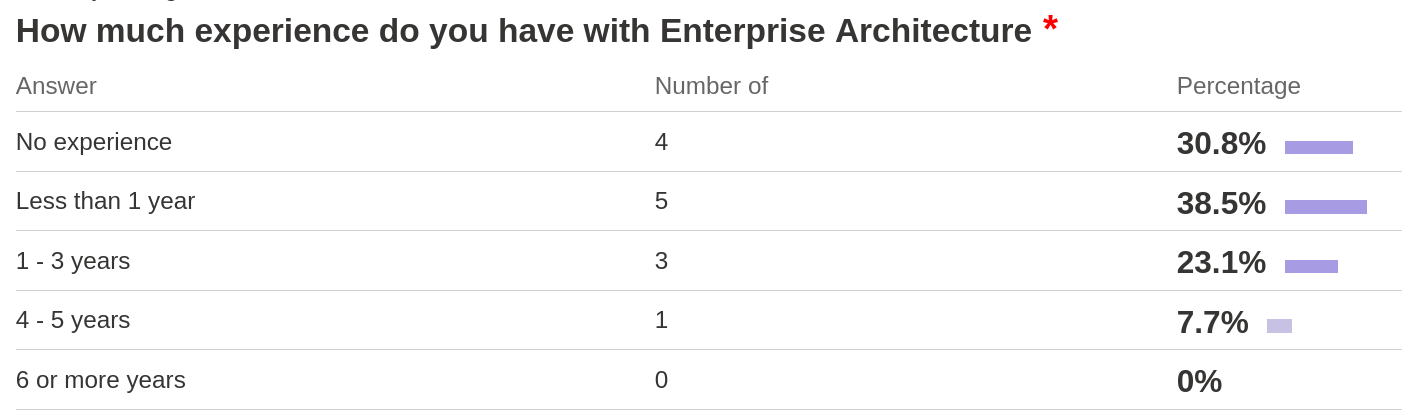
\includegraphics[scale=0.35]{figures/png/questionnaire_EA_Experience.png}
    \caption{Questionnaire demographic on EA experience}
    \label{fig:questionnaire-ea-experience}
\end{figure}

\begin{figure}
    \centering
    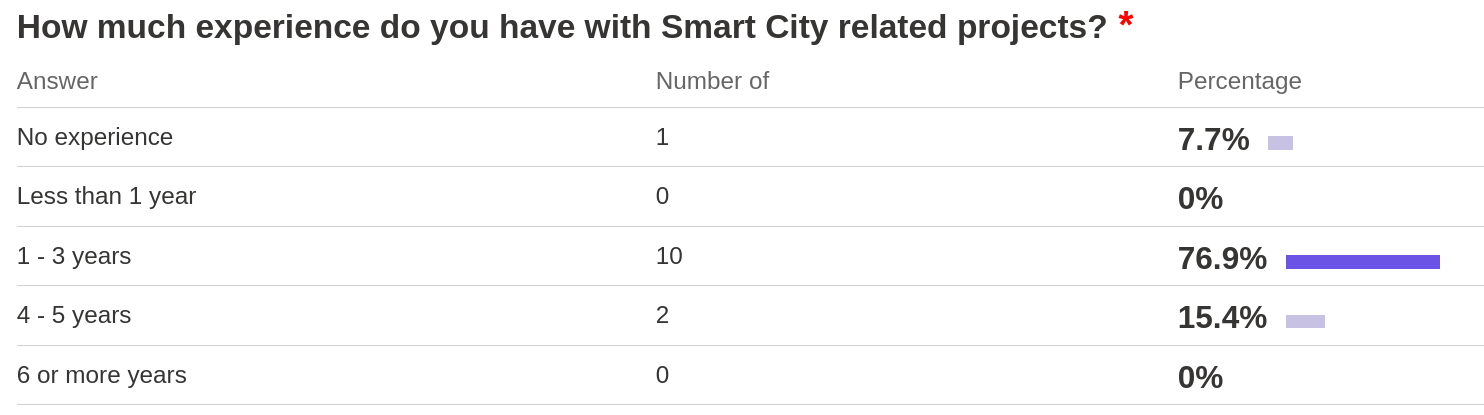
\includegraphics[scale=0.33]{figures/png/questionnaire_SmartCity_Experience.png}
    \caption{Questionnaire demographic on smart city experience}
    \label{fig:questionnaire-smartcity-experience}
\end{figure}



Figure \ref{fig:questionnaire-ea-experience} and \ref{fig:questionnaire-smartcity-experience} show the participants experience with \gls{ea} and smart city projects respectively. It shows that a significant percentage of participants have little experience with \gls{ea}. This makes it hard to trust some of the data in regards to quality of the \gls{eaf} and \gls{ea} model, but also shows the level of expertise of the users. It is clear that the models must be understood by those with little experience with \gls{ea}. The participants had more experience with smart city projects. This makes the domain specific questions more trustworthy. 

\subsection{Ease of use and usefulness}
The questionnaire results indicate that \gls{ea} in general and the +CityxChange \gls{eaf} in particular are seen as useful in the +CityxChange project, but the \gls{eaf} is not easy to understand. 

\subsection{How it relates to knowledge transfer}
The questionnaire results indicate that the \gls{eaf} could be useful for both retaining and sharing knowledge.

\subsection{Free-text answers}
Due to the nature of these questions, no statistical analysis was conducted. It is still seen that valuable information could be drawn from them. The answers indicate that the organisations vary greatly in how they approach knowledge retention and transfer and all of them use multiple approaches. The methods used include both formal and informal methods. Only one answer indicated that their organisation was considering changes or additional methods to retain or transfer knowledge within their organisation. This could indicate that most find their current methods satisfactory. 

Most answers indicated that their organisation did not use any other \gls{ea} approaches than the +CityxChange \gls{eaf}. One answer mentioned using \gls{togaf} while another mentioned an intention to use in the future, but that it was not relevant for +CityxChange. This could indicate that the +CityxChange \gls{eaf} covers its domain well and that modifying the \gls{eaf} for hybrid approaches is not of high importance.

The answers indicated that it was difficult to use without a background in \gls{ea} and that additional value could be gained from lowering the difficulty to a point were non practitioners could understand it. This could indicate that either the detail is too high, that the presentation is difficult to understand or the inherent complexity is problematic. The terminology used in the \gls{eaf} should be reconsidered or clarified.

The last specific question of the questionnaire was in regards to which problems the individual thought should be solved by \gls{ea}. The answers varied a lot with no discernible pattern. It is believed that the question was too broad, but the answers still brought forth a few sentiments that should be considered. A compilation of the answers would be; frameworks and tools for defining and implementing software architecture, aspects of data, regulatory compliance, knowledge retention, digital transformation, \gls{ict} system replication, high level view, cross organisational cooperation, complex systems and sharing of architectural knowledge.

\section{Extracted EA Requirements}
based on the questionnaire and literature, a few requirements were made for the \gls{eaf} and resulting \gls{ea} models.

\begin{itemize}
    \item The \gls{eaf} must be understandable based on the architecture alone for non technical personnel.
    \item The \gls{ea} models must be easy to understand for people with some experience with the \gls{eaf} without thorough understanding of the scenario it describes.
    \item The \gls{eaf} model must be improved with common knowledge retention, sharing and transfer activities in mind.
    \item The \gls{eaf} model must be improved with supplementary technologies in mind. 
    \item Describe which views could be useful for different supplementary activities.
\end{itemize}

\chapter{+CityxChange EAF evaluation}
This chapter presents an evaluation of the +CityxChange based on the literature review and information gathered from +CityxChange. 

\section{Evaluation based on data gathered from +CityxChange}
The evaluation presented in this section is informed by the survey presented in chapter \ref{chap:survey} and meeting notes. The meeting notes were taken during meetings between \gls{ea} architect and key personnel with an overview of the +CityxChange. The meetings were conducted to give feedback and correct deviations between \gls{ea} models created using the +CityxChange \gls{eaf} and their \gls{ict ecosystem}. 

\begin{itemize}[label=+]
    \item Its focus is relevant for the information that needs to be transferred.
    \item Goals and interests can be shown.
    \item Separate view can be used to mask information that is not important to individuals.
    \item External factors are considered.
    \item The representation covers the necessary parts of the system for development. 
\end{itemize}
\begin{itemize}[label=-]
    \item It is too complicated for beginners.
    \item The framework presentation can be confusing.
    \item The terminology can be confusing.
    \item The term "Business" has been criticised as being inappropriate when citizen welfare is a core motivator. 
    \item It is not designed with specific knowledge retention or knowledge sharing activities or methods in mind. 
    \item The focus is on the \gls{ict} system modelling and not on the human aspect.
\end{itemize}

\section{Evaluation based on Boundary objects perspective from literature}
The evaluation presented here is based on the \glspl{boundary object} properties described in \cite{abraham2015crossing};
\begin{itemize}
    \item \textbf{Accessibility:} The questionnaire indicate that complexity made it inappropriate as a communication channel with other communities than those experienced with \gls{ea}.  
    \item \textbf{Concreteness:} The questionnaire indicated that there was no information missing from the model that was desired by the respondents.  
    \item \textbf{Modularity:} The models layered architecture allow for high modularity.
    \item \textbf{Shared syntax:} Multiple respondents to the questionnaire requested revisiting the terminology, indicating that the syntax is flawed.
    \item \textbf{Annotation:} The model does not specifically encourage nor discourage annotation.
    \item \textbf{Visualization:} The current use of the model uses standard notations for \gls{togaf}. The representation of the \gls{eaf} itself has been noted as confusing. 
    \item \textbf{Malleability:} The complexity of the \gls{eaf} might prevent changes of the models without help of an \gls{ea} architect. 
    \item \textbf{Participation:} The meetings used to inform the model involved multiple communities, but the complexity of the \gls{eaf} might prevent direct change by the communities. 
    \item \textbf{Up-to-Dateness:} The \gls{eaf} does not specifically encourage nor discourage continuous change.   
\end{itemize}

\section{Evaluation based on Innovation perspective from literature}
The evaluation presented here is based on the innovation capabilities described in \cite{louw2017architecting}.
{\centering
\begin{longtable}{|p{2.5cm}|p{3cm}|p{8cm}|}
    \hline
    Sub architecture & Layer & Innovation capability \\ \hline
    \multirow{7}{2.5cm}{Horizontal layers} 
        & \multirow{42}{3cm}{Context} &  Proactive initiatives for identifying opportunities. \\  \cline{3-3}
        & & Procedures to manage and realise ideas. \\ \cline{3-3}
        & & Testing, screening and prioritising opportunities and ideas. \\ \cline{3-3}
        & & Ideas are quickly defined and prototyped. \\ \cline{3-3}
        & & Practices and procedures for developing and implementing ideas. \\ \cline{3-3}
        & & Practices to network and facilitate collaboration between internal teams. \\ \cline{3-3} 
        & & Procedures for identifying and exploring latent opportunities. \\ \cline{3-3}
        & & Core competencies are identified \\ \cline{3-3}
        & & Human resources are managed to ensure sufficient core competencies for operational needs. \\ \cline{3-3}
        & & Core innovation competencies are identified. \\ \cline{3-3} 
        & & Human resources are managed to ensure sufficient core competencies for research and development. \\ \cline{3-3}
        & & Procedures to ensure needed competencies are considered during the hiring process. \\ \cline{3-3} 
        & & Procedures for communication has been identified and implemented. \\ \cline{3-3} 
        & & Organisational resource needs are being monitored. \\ \cline{3-3}
        & & Sufficient resources are allocated to innovation. \\ \cline{3-3}
        & & Investment and prioritisation of innovation. \\ \cline{3-3}
        & & Organisational values and policies encourage innovation. \\ \cline{3-3}
        & & Change management procedures have been defined and deployed. \\ \cline{3-3}
        & & Initiatives for motivating, rewarding, and celebrating success. \\ \cline{3-3}
        & & Align existing personnel’s skills with their role. \\ \cline{3-3}
        & & Creating cross-functional and multidisciplinary teams. \\ \cline{3-3}
        & & Flexible organisational and human allocation structures. \\ \cline{3-3}
        & & Organisational structures that encourage organisation wide communication. \\ \cline{3-3}
        & & The organisational structure enables efficient decision-making. \\ \cline{3-3}
        & & Innovation metrics have been identified and defined. \\ \cline{3-3}
        & & Benchmarkings has been established to compare innovation metrics with successful organisations. \\ \cline{3-3}
        & & Goals are aligned with innovation objectives. \\ \cline{3-3}
        & & Innovation activities are appropriately prioritised with allocated resources.\\ \cline{3-3}
        & & Identifying and planning for important decisions. \\ \cline{3-3}
        & & Innovation process and activities are grounded in theory. \\ \cline{3-3}
        & & Innovation committee has been established or roles have been identified and assigned responsibility for key innovation related choices. \\ \cline{3-3}
        & & Identifying, documenting and implementing best-practices for innovation. \\ \cline{3-3}
        & & Identified strategy for knowledge acquisition. \\  \cline{3-3}
        & & Identified strategy for acquiring knowledge related technologies. \\  \cline{3-3}
        & & Strategy and innovation objectives are continuously improved and communicated. \\ \cline{3-3}
        & & Align project management with type(s) of innovation. \\ \cline{3-3}
        & & Innovation process competencies have been identified, acquired and developed. \\ \cline{3-3}
        & & Frameworks for contextualising, categorising and analysing data. \\ \cline{2-3}
        & \multirow{1}{3cm}{Services} & \textbf{Non} \\  \cline{2-3}
        & \multirow{1}{3cm}{Business} & \textbf{Non} \\  \cline{2-3}
        & \multirow{1}{3cm}{Application} & \textbf{Non} \\  \cline{2-3}
        & \multirow{6}{3cm}{Data Space} & Procedures for continuously understanding the needs of the end user. \\  \cline{3-3}
        & & Managing tacit knowledge. \\ \cline{3-3}
        & & Procedures for capturing, and retrieving data. \\ \cline{3-3}
        & & Practices for exploring existing and new fields of research. \\ \cline{3-3}
        & & Metrics are monitored to identify process and management improvements. \\ \cline{3-3}
        & & Procedures for identifying, summarising, highlighting, and extracting relevant information. \\ \cline{2-3}
        & \multirow{5}*{Technologies} & Core technologies are identified, managed, and maintained to ensure that project and operational needs are continuously fulfilled. \\ \cline{3-3}
        & & Procedures for proactively identifying, developing, and acquiring required technologies. \\ \cline{3-3}
        & & Tools to facilitate the information flow have been identified and implemented. \\ \cline{3-3}
        & & Tools for identifying, summarising, highlighting, and/or extracting relevant information. \\ \cline{3-3}
        & & Procedures for developing and elaborating concepts. \\  \cline{3-3}
        & & Tools and technology for storing and maintaining data. \\ \cline{2-3}
        & \multirow{1}*{Infrastructure} & Physical resources are allocated to the portfolio of projects, based on prioritisation and in balance with operational requirements.  \\ 
        \hline        
    \multirow{4}{2.5cm}{Stakeholder perspective} 
        & \multirow{3}{3cm}{Stakeholders} & Involving end user at various stages throughout the innovation process \\  \cline{3-3}
        & & Involving suppliers at various stages throughout the innovation process. \\ \cline{3-3}
        & & Involving other stakeholders (partners, alliances, etc.) in the innovation process. \\ \cline{2-3}
        & \multirow{2}{3cm}{Policies} & Procedures for ensuring supplier competency and that technology supports innovation type(s).\\  \cline{3-3}
        & & Practices to communicate and collaborate with external parties. \\ \cline{2-3}
        & \multirow{1}{3cm}{Privacy and Trust} & \textbf{Non} \\  \cline{2-3}
        & \multirow{1}{3cm}{Ownership} & Planning and coordinating the innovation portfolio. \\
         
        \hline        
    \multirow{3}{2.5cm}{Data Perspective} 
        & \multirow{1}{3cm}{Interoperability} & Opportunities and concepts are aligned and with required technology, competencies, processes, systems, etc.  \\  \cline{2-3}
        & \multirow{1}{3cm}{Data security, Risk} & Procedures to reduce project uncertainty and identify, manage, and mitigate risk. \\  \cline{2-3}
        & \multirow{3}{3cm}{Data Governance} & Managing and balancing the innovation portfolio. \\  \cline{3-3}
        & & Managing intellectual property. \\ \cline{3-3}
        & & Establish intellectual property management and sharing policy. \\ 
        \hline
    \multirow{6}{2.5cm}{Development process} 
        & \multirow{1}{3cm}{Identify component} & Opportunities and ideas are coordinated and viewed in context with required technology, competencies, processes, systems, etc.  \\  \cline{2-3}
        & \multirow{1}{4cm}{Identify relationships} & \textbf{Non} \\  \cline{2-3}
        & \multirow{1}{4cm}{Identify stakeholder} & \textbf{Non} \\  \cline{2-3}
        & \multirow{1}{3cm}{Validation} & \textbf{Non} \\  \cline{2-3}
        & \multirow{1}{3cm}{Iteration} & \textbf{Non} \\  \cline{2-3}
        & \multirow{1}{3cm}{Identify views} & \textbf{Non} \\
        \hline
    
    \caption{A mapping of the innovation capabilities discussed in \cite{louw2017architecting} table 1, to the +CityExchange EAF with changes to fit smart city development}
    \label{tab:4-innovation-capabilities}
\end{longtable}}
Table \ref{tab:4-innovation-capabilities} shows an attempt at mapping the innovation capabilities to the +CityxChange \gls{eaf}. Not all capabilities had a clear connection to each layer, therefore they were altered slightly and mapped to the best fit. Some of the capabilities could fit into multiple layers, showing that there might be an unintended overlap between the layers. Other capabilities did not fit well into any layer and where added to the closest layer based on terminology. This was often the case with capabilities surrounding procedures. Some of these procedures had clear ties to data, but did not fit into the data perspective or data layer while other related to policies. Many of the procedures that did not have a clear mapping was added to the context layer as that seemed to be the best fit. 

The mapping indicates that procedures are an important aspect of enterprises and innovation or learning, and are not explicitly covered by the \gls{eaf}. The mapping also indicate that the context layer is overworked. 
\chapter{Proposed model}
\label{chap:model}
This section describes the proposed enhancements to the  +CityxChange \gls{eaf} to promote learning across cities in smart city development projects.
\section{Developed model} % or framework/tool/system add subsection by need

When developing the new model, as many issues as possible, from the original, should be solved. But there is a trade-off between complexity and coverage. Complexity should be low to encourage use by non-experts while coverage should be high to allow use in multiple situations and for correct usage. 

\subsection{Enhancements of the development process}
\begin{figure}
    \centering
    \makebox[\textwidth][c]{
        \rotatebox{-90}{
            %New development process
% Define block styles
\tikzset{
    decision/.style={diamond, draw, fill=blue!20, text centered, text width = 1.5cm},
    block/.style={rectangle, draw, fill=blue!20, rounded corners, text width = 1.8cm},
    mindset/.style={
        rectangle split, rectangle split parts=2, 
        rectangle split part fill={yellow!20,green!20},
        draw, text width=2.4cm},
    to/.style={draw, -latex},
    connect/.style={draw, dashed},
    textnode/.style={text width=0.5cm}
}

    
\begin{tikzpicture}[]
    % Main steps
    \node[block, left= 0.8cm of components] (users) {Consider users interested in this model};
    \node [block] (components) {Identify and describe components in horizontal layers};
    \node [block, right= 0.8cm of components] (documentation) {Identify documentation and knowledge reservoirs};
    \node[block, right= 0.8cm of documentation, yshift=1.2cm] (resources) {Identify and describe resources};
    \node [block, right= 0.8cm of documentation, yshift=-1.2cm] (relationships) {Identify and describe relationships};
    \node [block, right= 0.8cm of relationships, yshift=1.2cm] (perspectives) {Identify stakeholder and data perspectives};
    \node [decision, right= 0.5cm of perspectives] (iscomplete) {Is model complete};
    \node [block, above= 0.5cm of resources] (iterate) {Iterate to add detail};
    \node [block, right= 0.6cm of iscomplete] (views) {Identify views to visualise};

    % Mindset
    \node[mindset, below=0.8cm of users] (mindusers) { \nodepart{one} \begin{center} Mindset \end{center}
        \nodepart{two}
        \begin{itemize}[leftmargin=0.3cm]
            \item Why is the model needed?
            \item Who is the model for?
        \end{itemize}
    };
    
    \node[mindset, below=0.8cm of components] (mindcomponents) { \nodepart{one} \begin{center} Mindset \end{center}
        \nodepart{two}
        \begin{itemize}[leftmargin=0.3cm]
            \item What is relevant for the models users?
            \item What is needed to make decisions?
            \item How does the \gls{ea} look to outsiders?
        \end{itemize}
    };
    
    \node[mindset, below=0.8cm of documentation] (minddocumentation) { \nodepart{one} \begin{center} Mindset \end{center}
        \nodepart{two}
        \begin{itemize}[leftmargin=0.3cm]
            \item Where can users find more information?
            \item What documentation needs to be updated on changes?
        \end{itemize}
    };
    
    \node[mindset, below=0.8cm of relationships] (mindrelationships) { \nodepart{one}
    \begin{center} Mindset \end{center}
        \nodepart{two}
        \begin{itemize}[leftmargin=0.3cm]
            \item Who and what is communicated?
            \item Which protocols or processes do they use?
            \item Which techniques are used to share/retain knowledge?
            \item How is communication documented?
        \end{itemize}
    };
    
    \node[mindset, below=0.8cm of perspectives] (mindperspectives) { \nodepart{one}
    \begin{center} Mindset \end{center}
        \nodepart{two}
        \begin{itemize}[leftmargin=0.3cm]
            \item Who has an interest in the systems completion?
            \item Who participates in development?
        \end{itemize}
    };
    
    \node[mindset, below=0.8cm of views] (mindviews) { \nodepart{one}
    \begin{center} Mindset \end{center}
        \nodepart{two}
        \begin{itemize}[leftmargin=0.3cm]
            \item Do groups interpret the system differently?
            \item Do groups have different terminology?
            \item Are there things that are likely to be misinterpreted?
            \item Can unnecessary information be hidden?
        \end{itemize}
    };
    
    \node[mindset, below=1.5cm of iscomplete] (mindresources) { \nodepart{one}
    \begin{center} Mindset \end{center}
        \nodepart{two}
        \begin{itemize}[leftmargin=0.3cm]
            \item Have human resources been allocated?
            \item Have financial resources been allocated?
            \item Are there missing resources?
            \item Could resources improve the system?
        \end{itemize}
    };
    
    % Draw flow
    \path [to] (users.east) -- (components.west);
    \path [to] (components.east) -- (documentation.west);
    \path [to] (documentation.east) -| (4.3,-1.2) -- node [below, xshift=-0.2cm] {And} (relationships.west);
    \path [to] (documentation.east) -| (4.3,1.2) -- node [above, xshift=-0.2cm] {And} (resources.west);
    \path [to] (relationships.east) -| (7,0) -- (perspectives.west);
    \path [to] (resources.east) -| (7,0) -- (perspectives.west);
    \path [to] (perspectives.east) -- (iscomplete.west);
    \path [to] (iscomplete.north) |- node [right] {no} (iterate.east);
    \path [to] (iterate.west) -| (components.north);
    \path [to] (iscomplete.east) -- node [above] {yes} (views.west);
    
    % Draw supplimentary connections
    \path[connect] (users) -- (mindusers);
    \path[connect] (components) -- (mindcomponents);
    \path[connect] (documentation) -- (minddocumentation);
    \path[connect] (relationships) -- (mindrelationships);
    \path[connect] (perspectives) -- (mindperspectives);
    \path[connect] (views) -- (mindviews);
    \path[connect] (resources.north) |- (10, 2.5) |- (mindresources.north west);
\end{tikzpicture}


        }
    }
    \caption{Development process of an EA using the proposed model.}
    \label{fig:4-architecture-development-after}
\end{figure} %Collaboration layer
% Identify <Conspets>
% Component, entity Explain
% Explain mindset


The development process of an \gls{ea} has been altered, as shown in figure \ref{fig:4-architecture-development-after}, to allow for consideration of elements that are relevant to learning. It is meant as a guide and not meant to be used as a hard requirement. More specifically; three steps have been added.
\begin{itemize}
    \item \textbf{Consider users}: Added due to learning and \gls{ea} being concepts that are intrinsically linked to human efficiency and behaviour.
    \item \textbf{Knowledge identification}: Added as it is believed that the \gls{ea} model by itself will not be able to sufficiently cover everything each individual needs for learning, but can still guide the individual towards important information. It also forces the \gls{ea} architects to consider how knowledge is created within the system.
    \item \textbf{Resource identification}: Added due to resources being a concept that is repeatedly mentioned in the literature. Both when it comes to innovation and within smart city development due to the multi stakeholder context.
\end{itemize}

{\centering
\begin{longtable}{|p{6cm}|p{6cm}|}
    \hline
    Mindset & Relevant \gls{boundary object} properties \\ \hline
    Why is the model needed? & concreteness\\ \hline
    Who is the model for? & concreteness, malleability, participation \\ \hline

    What is relevant for the models users? & concreteness, malleability, participation\\ \hline
    What is needed to make decisions? & concreteness \\ \hline
    How does the \gls{ea} look to outsiders? & concreteness\\ \hline

    Where can users find more information? & concreteness, (indirect) accessibility \\ \hline
    What documentation needs to be updated on changes? &  Up-to-dateness \\ \hline

    Who and what is communicated? & concreteness \\ \hline
    Which protocols or processes do they use? & concreteness \\ \hline
    Which techniques are used to share/retain knowledge? & concreteness \\ \hline
    How is communication documented? & concreteness\\ \hline

    Who has an interest in the systems completion? & concreteness, malleability, participation \\ \hline
    Who participates in development? & concreteness, malleability, participation \\ \hline

    Do groups interpret the system differently? & shared syntax, annotation, modularity\\ \hline
    Do groups have different terminology? & shared syntax \\ \hline
    Are there things that are likely to be misinterpreted? & shared syntax \\ \hline
    Can unnecessary information be hidden? & modularity, visualization\\ \hline
    
    Have human resources been allocated? & concreteness \\ \hline
    Have financial resources been allocated? & concreteness, visualization \\ \hline
    Are there missing resources? & concreteness, visualization \\ \hline
    Could resources improve the system? & concreteness, visualization \\ \hline
    
    \caption{A mapping of the mindsets to relevant Boundary object properties}
    \label{tab:4-mindset-properties}
\end{longtable}}
Figure \ref{fig:4-architecture-development-after} also adds questions one can have in mind while developing the \gls{ea} model. The questions are called mindsets and are meant to make the intention behind the \gls{ea} model clearer to the architect and make them consider knowledge flows. A mindset in this context is a perspective or set of ideas that can influence decisions. This semi-structured approach is used as the concept of "learning" is hard to define or achieve in a rigid environment. The mindsets are a result of viewing the \gls{ea} model as a \gls{boundary object}, It does not use the specific terminology within the diagram, as it is not expected that the \gls{ea} architects are familiar with the concept. Table \ref{tab:4-mindset-properties} shows how the terminology applies to the mindsets. 

\subsection{Enhancements of the EAF}
\begin{figure}
    \centering
    %\begin{turn}{-90}
    \makebox[\textwidth][c]{
        \tikzset{
  box/.style={
    draw,
    rectangle,
    minimum height=1cm,
    fill=white,
    align=center,
    inner sep=1ex
  }
}

\begin{tikzpicture}[]
    \iffalse
    \begin{scope}[on background layer]
         \node at (-0.5,-3) [box, minimum width=2.5cm, text width=1.8cm, minimum height=9cm, fill=cyan, align=north] (planning) {Integrated Planning and design};
        \node[box, minimum width=2.5cm, text width=1.8cm, minimum height=9cm, fill=cyan, right= 2mm of planning] (common) {Common energy market};
        \node[box, minimum width=2.5cm, text width=1.8cm, minimum height=9cm, fill=cyan, right= 2mm of common] (community) {Community- xChange};   
    \end{scope}
    \fi
    %Horizontal - Inner
    \node[box, opacity=0.8, text width=\textwidth/2]  (process) {processes and internal initiatives};
    \node[box, opacity=0.8, text width=\textwidth/2, below=2mm of process]  (team) {Team structures};
    \node[box, opacity=0.8, below=2mm of team, text width=\textwidth/1.8]  (goal) {Goals and KPIs};
    \node[box, opacity=0.8, below=2mm of goal, text width=\textwidth/2] (service) {Value Added Services};
    \node[box, opacity=0.8, below=2mm of service, text width=\textwidth/2]  (business) {Enterprise cooperation};
    \node[box, opacity=0.8, below=2mm of business, text width=\textwidth/2]  (application) {Application and Data Processing};
    \node[box, opacity=0.8, below=2mm of application, text width=\textwidth/2]  (data) {Data Space};
    \node[box, opacity=0.8, below=2mm of data, text width=\textwidth/2]  (technology) {Technologies};
    \node[box, opacity=0.8, below=2mm of technology, text width=\textwidth/2]  (physical) {Physical Infrastructure};

    % Context - Outer
    \begin{scope}[on background layer]
        \node[box, opacity=0.1, inner sep=1ex, fit=(process) (team) (goal) (service) (business) (application) (data) (technology) (physical)] (main) {};
    \end{scope}

    % Stakeholder perspective  - Inner
    \node[box, minimum height=\textwidth/2, left=of main] (ownership) {\rotatebox{90}{Ownership and access}};
    \node[box, minimum height=\textwidth/2, left=2mm of ownership] (privacy) {\rotatebox{90}{Privacy \& Trust}};
    \node[box, minimum height=\textwidth/2, left=2mm of privacy] (policy) {\rotatebox{90}{Policies \& Regulations}};
    \node[box, minimum height=\textwidth/2, left=2mm of policy] (stakeholder) {\rotatebox{90}{Stakeholders}};

    % Stakeholder perspective  - Outer
    \begin{scope}[on background layer]
        \node[box, inner sep=1ex, fit=(stakeholder) (policy) (privacy) (ownership),  label={Stakeholder perspective}] (stakeholder) {};
    \end{scope} 

    % Data perspective - Inner    
    \node[box, minimum height=\textwidth/2, right=of main] (interoperability) {\rotatebox{90}{interoperability}};
    \node[box, minimum height=\textwidth/2, right=2mm of interoperability] (security) {\rotatebox{90}{Data security, Risk assessment}};
    \node[box, minimum height=\textwidth/2, right=2mm of security] (governance) {\rotatebox{90}{Data Governance}};
    
    % Stakeholder perspective  - Outer
    \begin{scope}[on background layer]
        \node[box, inner sep=1ex, fit=(interoperability) (security) (governance),  label={Data perspective}] (stakeholder) {};
    \end{scope} 

\end{tikzpicture}
    }%
    %\end{turn}
    \caption{Proposed EAF based on the +CityxChange EAF}
    \label{fig:4-architecture-after}
\end{figure}


As shown in figure \ref{fig:4-architecture-after} and \ref{fig:4-architecture-elements} the \gls{eaf} has been expanded and more architectural elements have been added. Although this could intuitively increase complexity, the intent is that a further segmentation of the domain and greater specificity with better concreteness, shared syntax and visualization, can make the model more intuitive and allow more relevant views for individuals. 

The original context layer has been expanded to three layers; "goals and \glspl{kpi}", "Team structures" and "processes and internal initiatives". The "goals and \glspl{kpi}" layer is intended to be used like the context layer was used in the original. It contains the core motivations behind the system(s) being developing. Figure \ref{fig:4-architecture-after} shows this layer being accentuated. This is because it is considered to be vital for decision making. "Team structures" and "Processes and internal initiatives" were placed above, not because of higher significance, but because they are further removed from the application and physical infrastructure layers. The added "Team structures" layer is for documenting internal teams working on development. It is intended to help understand how knowledge flows between people and groups. It is different from the layer in the origin \gls{eaf} called "Business (Virtual Enterprise)" and called "Enterprise collaboration" in the proposed \gls{eaf} in that the collaboration layer contains companies or stakeholders involved in the development rather than internal structures that might be specific to each stakeholder. "Processes and internal initiatives" is the final layer that has been changed from the original. It is meant to capture more of the knowledge flows by adding processes that are initiated and heavily governed by peoples, such as daily meetings and workshops. 

\subsection{Addition EA elements}
\begin{figure}
    \centering
    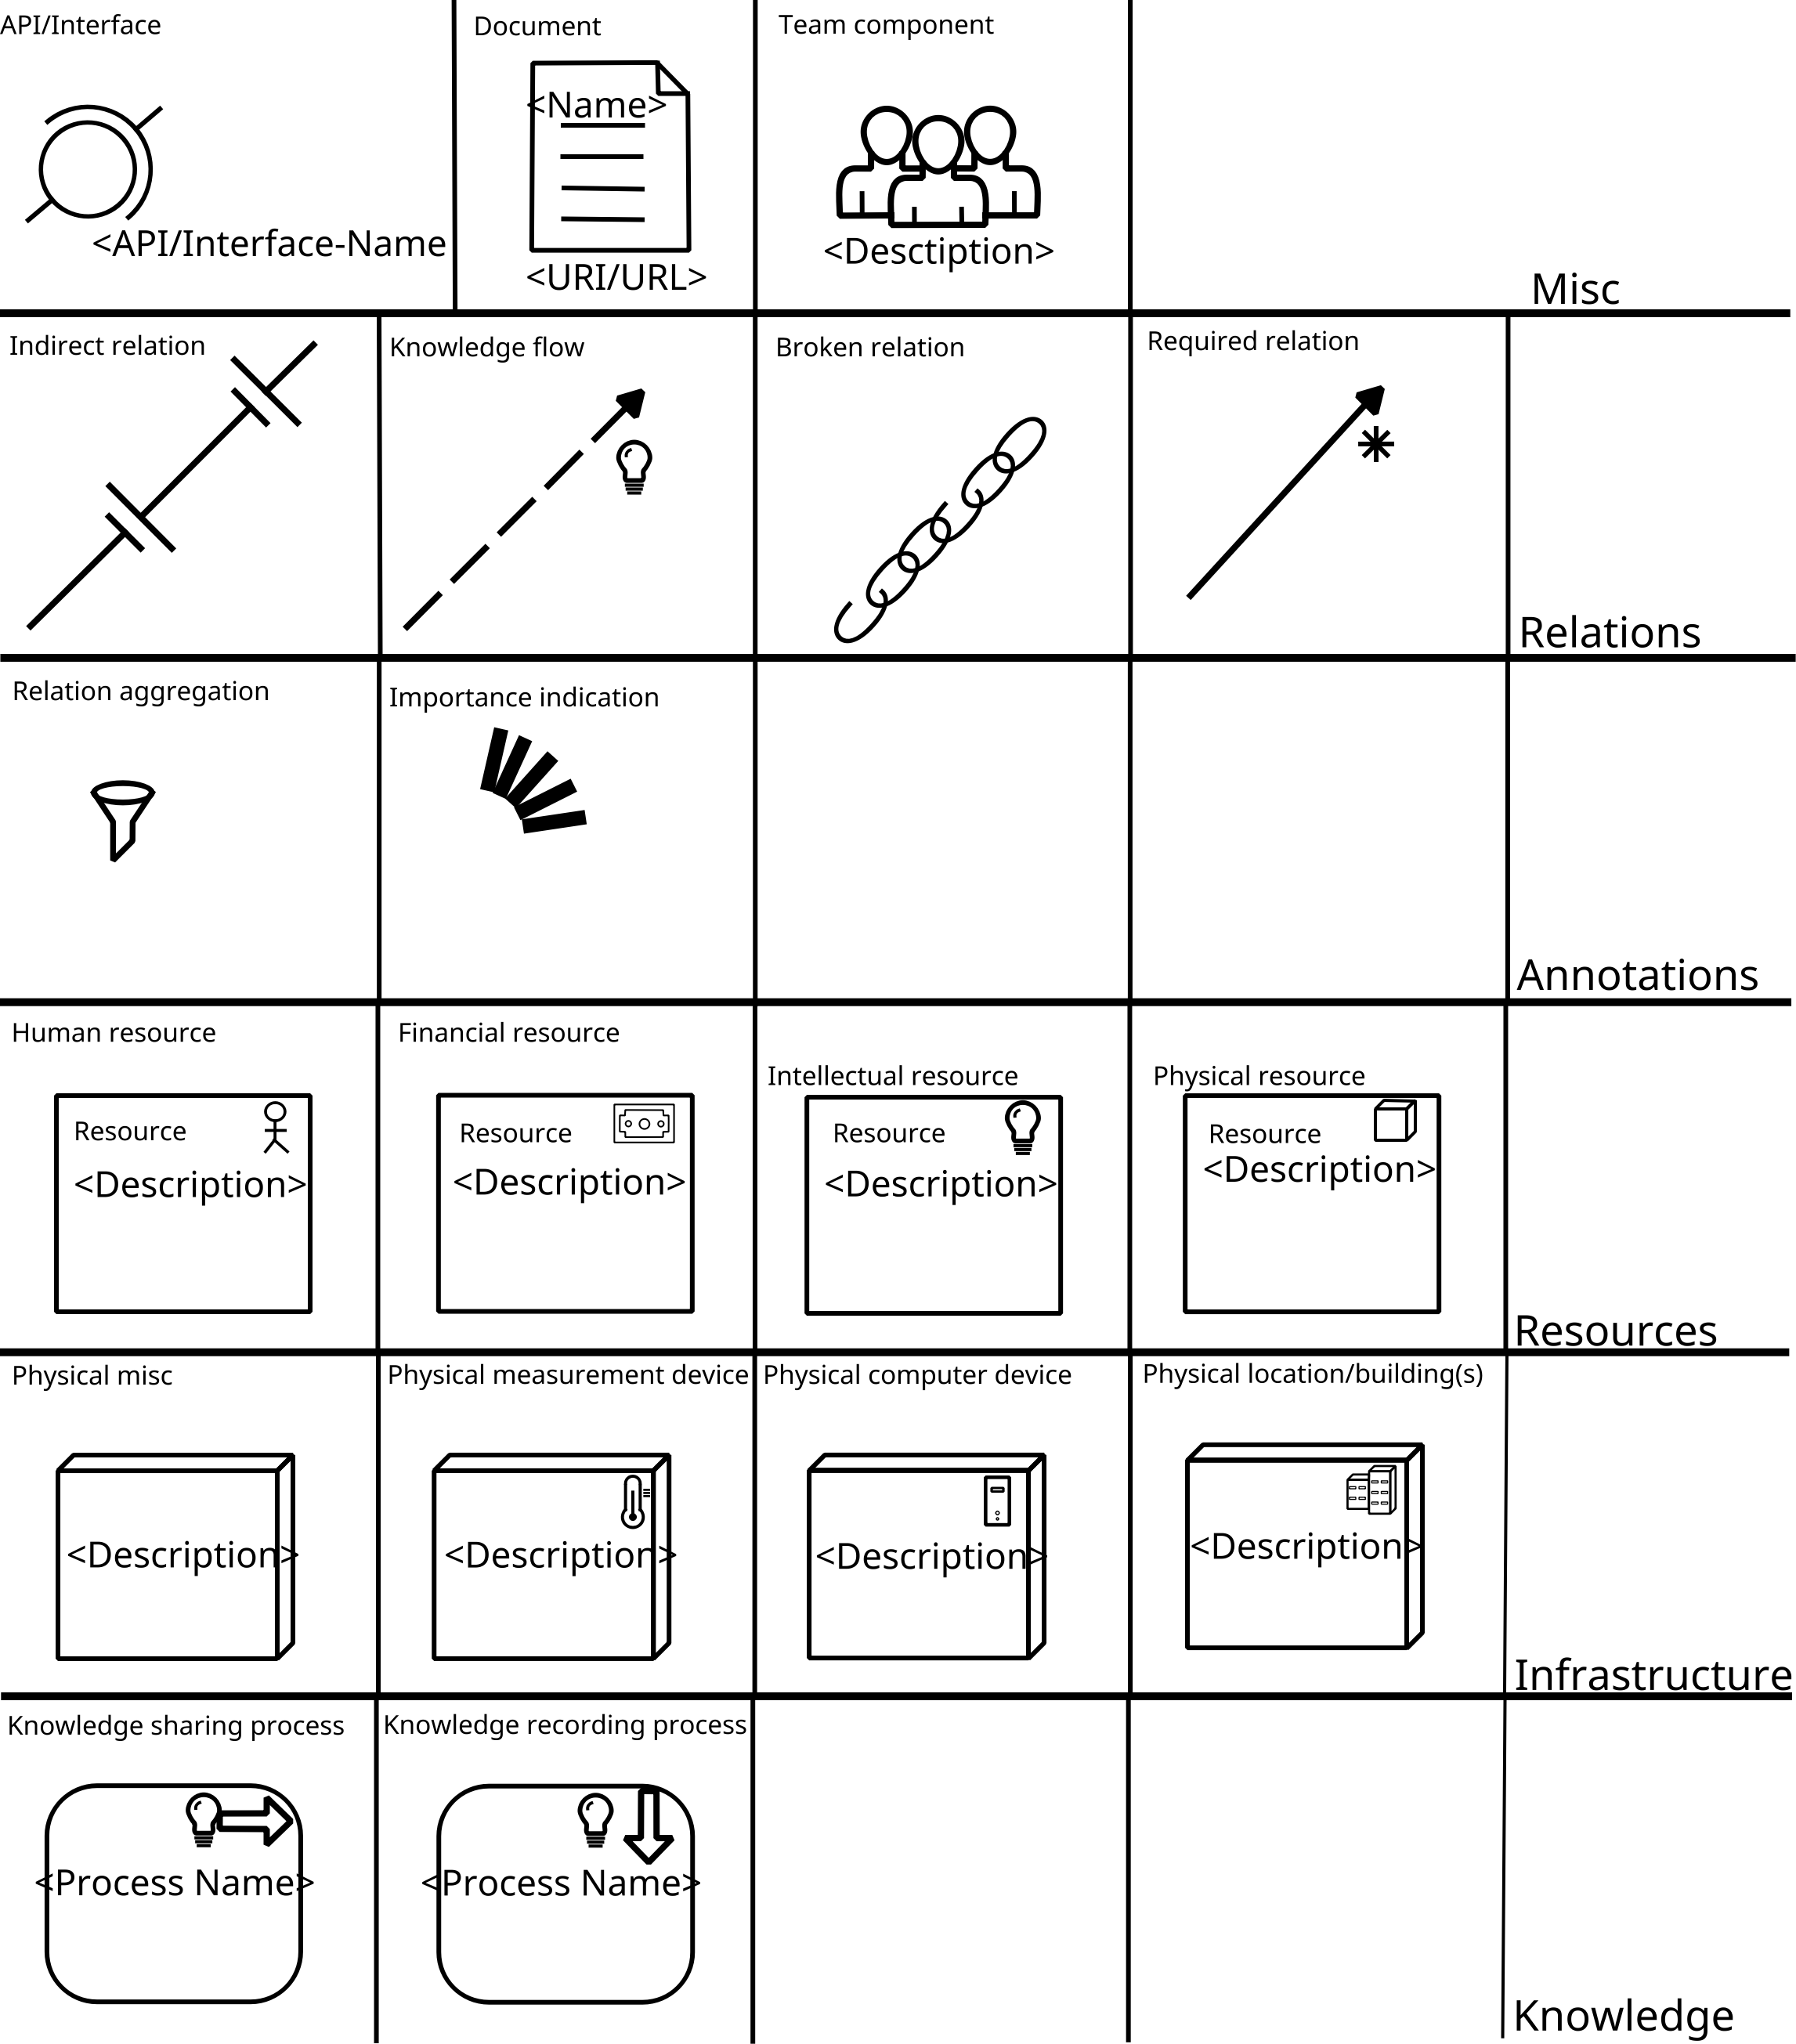
\includegraphics[scale=0.6]{figures/png/elements.png}
    \caption{Proposed elements for making EA models from proposed EAF }
    \label{fig:4-architecture-elements}
\end{figure}

Figure \ref{fig:4-architecture-elements} shows the proposed elements that can be used to create the \gls{ea} models. It is meant to supplement or enhance the elements in \gls{togaf}. \gls{togaf} was used as a base due to its current use within +CityxChange and recommendation by multiple relevant articles \cite{7580810, pourzolfaghar2016types}.
Some of the elements, such as aggregation and indirect connections, have been added to allow views to partially be created logically from a base \gls{ea} model allowing further hiding of irrelevant information. while other elements are meant to include knowledge related components or better represent the smart city context.

\begin{itemize}
    \item \textbf{Api/interface} element is an alteration of the \gls{togaf} interface elements. It has been changed so that it is more clearly differentiated from the other elements. This was done as the \glspl{api} were a topic mentioned repeatedly in +CityxChange meetings and are seen as important parts of the \gls{ea}.
    \item \textbf{Document} element is a  more general version of \gls{togaf} artefact that also has a \gls{url}/\gls{uri}. This \gls{url}/\gls{uri} was added to improve the accessibility of the document.\Gls{the open group} defines an artefact as "a physical piece of data that is used or produced in a software development process, or by deployment and operation of a system."\cite{archilayer}. The proposed document is not tied to the software, but can be things like meeting notes.
    \item \textbf{Team component} was added because humans are the core of any knowledge related activity.
    \item \textbf{Indirect relation} was added to allow hiding of connected elements in certain views without hiding the connections between the other elements.
    \item \textbf{Knowledge flow} shows how knowledge flows in the \gls{ea} and was added to make knowledge information more specific.
    \item \textbf{Broken relation} shows that a connection is expected or preferred, but not implemented. This was added to visualise potential areas for improvement or innovation.
    \item \textbf{Required relation} shows that a connection can not be removed without significant work. This was added to allow separate communities to give additional information about what is necessary from their perspective.
    \item \textbf{Relation aggregation} was added as the multi stakeholder context often require many to one connections and a way to remove clutter could improve visualisation. It might also be beneficial for views where components with several connections are hidden. 
    \item \textbf{Importance indicator} is meant to attach to other components to indicate that the user of the \gls{ea} model might want to consider that component. It can be relevant to add this to specific views as importance is dependent on perspective.
    \item \textbf{Resources} elements expand the \gls{togaf} resource element with four more specific version and a new notation. The versions are human financial, intellectual and physical resources respectively. These were added based on their importance for innovation capabilities.
    \item \textbf{Physical entities} were added as the smart city concept often revolve around physical infrastructure such as chargers for \gls{emaas}, sensors for data gathering and smart grids. The \gls{togaf} node element is changed into a physical misc element for generic physical components and specific elements were added for measurement, computation devices and locations.
    \item \textbf{Knowledge processes} were added to show how the knowledge flows within the \gls{ea}, how it is shared and how it is recorded.
\end{itemize}
 
Some of the unchanged elements from \gls{togaf} that are seen as important are; the influence relation, the stakeholder and goals/\gls{kpi} related elements, principle element and note. 
{\centering
\begin{longtable}{|p{2.3cm}|p{4.5cm}|p{5cm}|}
    \hline
        Grouping & Element & Description/attribute\\ \hline
        \multirow{3}*{Misc} 
            & \multirow{4}*{API or interface} & Used to indicate \gls{api} or interfaces. \\ \cline{3-3}
            & & Attribute: \gls{api} name. \\ \cline{3-3}
            & & Attribute: \gls{api} ID for lookup. \\ \cline{3-3}
            & & Attribute: File link or \gls{uri}. \\ \cline{2-3}
            & \multirow{7}*{Document} & Used to represent documentation or artefact stored outside the current \gls{ea} model. \\ \cline{3-3}
            & & Can be used refer to other \gls{ea} components, \gls{uml} diagram, organisational charts, system specifications, resource allocations, etc. \\ \cline{3-3}
            & & Attribute: File name. \\ \cline{3-3}
            & & Attribute: File description. \\ \cline{3-3}
            & & Attribute: File link or \gls{uri}. \\ \cline{3-3}
            & & Attribute: File access description (if link or \gls{uri} is not applicable). \\ \cline{3-3}
            & & Attribute: File type or comprehension. \\ \cline{2-3}
            & \multirow{1}*{Organisational component} &  Used to represent a team, group or other organisational structure. \\
        \hline
        \multirow{4}*{Relations} 
            & \multirow{1}*{Indirect relation} &  Used to show an indirect relationship that should be known. \\  \cline{2-3}
            & \multirow{1}*{Knowledge flow} & Used to show how knowledge flows or is created. \\ \cline{2-3}
            & \multirow{1}*{Broken relation} & Used to show that a relation is expected, but not implemented or functional. \\ \cline{2-3}
            & \multirow{1}*{Required relation} & Used to show that a relationship can not be removed. \\
        \hline
        \multirow{2}*{Annotation}
            & \multirow{1}*{Relation aggregation} &  Used to simplify visualisation of many to one or many to many relationships. \\ \cline{2-3}
            & \multirow{2}*{Importance indicator} &  Used to show that a component or relation is important for development or decision making. \\ \cline{3-3}
            & & Attribute: Justification \\
        \hline
        \multirow{4}*{Resources}
            & \multirow{5}*{Resource misc} & Used to represent a resource, when no other element can be more descriptive. \\ \cline{3-3}
            & & Attribute: Resource type. \\ \cline{3-3}
            & & Attribute: Resource quantity. \\ \cline{3-3}
            & & Attribute: Resource description. \\ \cline{3-3}
            & & Attribute: Resource justification.\\ \cline{2-3}
            & \multirow{4}*{Human Resource} & Used to represent a human resource. \\ \cline{3-3}
            & & Attribute: Resource quantity. \\ \cline{3-3}
            & & Attribute: Resource description. \\ \cline{3-3}
            & & Attribute: Resource justification.\\ \cline{2-3}
            & \multirow{4}*{Intellectual Resource} & Used to represent a knowledge based resource. \\ \cline{3-3}
            & & Attribute: Resource quantity. \\ \cline{3-3}
            & & Attribute: Resource description. \\ \cline{3-3}
            & & Attribute: Resource justification.\\ \cline{2-3}
            & \multirow{4}*{Physical Resource} & Used to represent a resource with physical properties. \\ \cline{3-3}
            & & Attribute: Resource quantity. \\ \cline{3-3}
            & & Attribute: Resource description. \\ \cline{3-3}
            & & Attribute: Resource justification.\\ \cline{2-3}
        \multirow{4}*{Infrastructure} 
            & \multirow{1}*{Physical misc} & Used to represent a physical entity when no other element is more descriptive. \\ \cline{3-3}
            & & Attribute: Type. \\ \cline{3-3}
            & & Attribute: Description. \\ \cline{2-3}
            & \multirow{1}*{Physical measurement device} & Used to represent data-gathering devices. \\ \cline{3-3}
            & & Attribute: Data type. \\ \cline{3-3}
            & & Attribute: Description. \\ \cline{2-3}
            & \multirow{1}*{Physical computation device} & Used to represent computing devices, servers or similar. \\ \cline{3-3}
            & & Attribute: Capability. \\ \cline{3-3}
            & & Attribute: Description. \\ \cline{2-3}
            & \multirow{1}*{Physical location/building} & Used to represent important locations or buildings. \\ 
        \hline
        \multirow{2}*{Knowledge} 
            & \multirow{1}*{Knowledge sharing process} & Used to represent activities such as meetings, workshops etc that share knowledge between individuals or groups. \\ \cline{3-3}
            & & Attribute: Process name. \\ \cline{3-3}
            & & Attribute: Knowledge description. \\ \cline{2-3}
            & \multirow{1}*{Knowledge recording process} & Used to represent activities such as document writing, meeting recording etc that result in tacit knowledge being converted to explicit knowledge. \\ \cline{3-3}
            & & Attribute: Process name. \\ \cline{3-3}
            & & Attribute: Knowledge description. \\
    \hline
    
    \caption{Suggested elements represented in the EA model and optional attributes of those.}
    \label{tab:4-element-attributes}
\end{longtable}}

Table \ref{tab:4-element-attributes} shows a more detailed view of the suggested elements. It adds attributes on some elements that might not be visible on the component, but can be added in a digital representation and viewed when a component is selected.  

\section{Summary}
This chapter presented an enhanced \gls{eaf} along with a \gls{ea} development process and \gls{ea} elements that can be used to represent an \gls{ea} that could support the transfer of learning across cities. The model builds on the +CityxChange \gls{eaf} and \gls{togaf}, and is intended to promote learning in a smart city context.
\chapter{Model evaluation}
\label{chap:evaluation}
\section{Purpose of evaluation}
An evaluation of the proposed model was performed to find out if the proposed changes were beneficial for smart city projects and could enhanced learning. 

\section{Interview findings}
Participant 1 was positive to how the elements and development process related to the \gls{eaf}, but had concerns about the \gls{eaf} itself. The participant mentioned that the distinction between "Enterprise cooperation" layer and "Team structures" was not clear and that the motivation for adding "Team structures" was not clear either. "Team structures" and "internal processes" seemed to be ill fit for multi stakeholder systems such as +CityxChange and did not inherently seem to be related to theories found in \gls{togaf} or similar frameworks. It seems that these two layers were trying to model the system on a different level then the other layers and could cause conflicts. An example that could cause conflict were if the "Goals and \glspl{kpi}" layer contained a goal, then it would be hard to note if the goal was connected to the internal teams in the layers above or the "Enterprise cooperation" layer. It was also unclear if the context layer was sufficiently covered by the three layers the proposed model replaced it with. Participant 3 also mentioned the importance of the context layer as it relates to learning. Participant 3 mentioned that "Goals and \glspl{kpi}" seemed to be for quantitative aspects, but lacked the qualitative aspects of context.

"Team structures" was mentioned by participant 1 as not being particularly important, that the important parts for +CityxChange were responsibilities and decisions. Participant 2 also mentioned that they did not see the motivation behind "Team structures" and elaborated on how it clashed with the over aching goals of the \gls{eaf} to model the cooperation between the partners and stakeholders while allowing the individual partners to steer their own development process. Participant 2 mentioned that if "Team structure" and "Processes and internal initiatives" were added, then they were more likely to be vertical layers similarly to "Stakeholder perspective". The layers could still be relevant but seemed to be misplaced. Participant 3 viewed "Team structures" as what they would consider "Institutional aspects". Although participant 2 and 3 both had issues with the layer, they also mentioned that it was important in some cases.

Participant 3 went into more detail on "Processes and internal initiatives". It was considered to be very important for learning, but also very complicated with many factors. They expect that the \gls{ea} model would have to overlook important aspects of learning related processes. Participant 3 also mentioned that peoples cultures or backgrounds would have a significant effect on processes and learning.

In regards to the suggested development process, participant 2 was mostly positive, but found the concept of "mindset" to be easily misunderstood. The idea behind it was still good, but other terminology should be considered. The specific questions listed in the mindsets were relevant, but seemed more relevant for evaluating existing architectures or understanding the motivation behind the components included in a finished model. Participant 3 mentioned that several steps and vocabulary was overlapping. As an example, it would be difficult to separate users of the model from stakeholders. This would also be a problem when developing the \gls{ea} model as it is usually developed by reading documentation and interviewing users or stakeholders. It was not clear from the development process who to communicate with and how they affect your mindset.

Participant 2 went into more detail than participant 1 when evaluating the proposed elements. Altering the interface element as suggested was not recommended, but they requested adding variants or notations to specify more details about \glspl{api}. For instance, there might be an \gls{api} that will exist in the future, an anonymous \gls{api} or request format. The "indirect relationship" was seen as problematic, as everything would in some way be indirectly connected and the graphical parts seemed like a poor visualisation of indirect relationships. It was also recommended to change the "broken relationship" visualisation as the more intricate notation made it seem like a stronger connection rather than broken. Adding more relationship notations was still seen as a good idea. Participant 2 thought the idea behind the resource elements were good, but only relevant at too high a detail for an \gls{ea} that was meant for a higher level view. Participant 3 also mentioned that the resulting model would likely be too complicated to be useful for most people. For the physical elements participant 2 requested that the "physical location/building" should allow for nesting while the "measurement device" should be a collection of devices and should have a different notation. A thermometer was not seen as appropriate for the "measurement device". Participant 2 mentioned that the knowledge elements would probably not be relevant because they would need to model at too fine a detail.
\chapter{Results and discussion}
\label{chap:result}
This section describes the results of the research and discusses how it relates to earlier work. It also covers shortcomings and possible sources for errors.

\section{Findings for \textbf{RQ1:} How is EA currently being used to enhance learning in smart city projects?}
The literature review found that most \gls{ea} used in \gls{ict} city planning does not specifically consider learning to a great extent. The literature is conflicted on whether or not \gls{ea} in smart city projects should be used to allow replication or should focus on flexibility. The literature suggests either \gls{ict} architectures when advocating replication or existing \glspl{eaf} when advocating flexibility. Most of the research using existing \glspl{eaf} suggests using \gls{adm} and a few suggests using zachman. 
Although most literature does not specifically relate to learning, it does suggest that \gls{adm} and other \glspl{eaf} cover important aspects of it. In particular the business aspects from the different \glspl{eaf} are seen as important. The survey indicate that the \gls{eaf} used in +CityxChange has high relevance to the project which is considered to be a key factor in \glspl{boundary object}. 
The complexity of the +CityxChange \gls{eaf} is a significant hindrance for learning. The research in this thesis could not determine if this was a result of the \gls{eaf} itself or inherent to \gls{adm} that it builds on or \gls{ea} in general. The suggested changes in the proposed model were unable to lower complexity or show any significant improvement in learning.

\section{Findings for \textbf{RQ2:} How can cities benefit from EA documentation of working smart city solutions?}
The literature is split on whether or not replication is achievable, but it is clear that \gls{ea} is part of the solution. Literature on \glspl{boundary object} shows that \glspl{boundary object} such as \gls{ea} models can be useful for learning as long as the information is closely related to the domain of interest where the learning takes place. The proposed model suggested adding information on internal teams, knowledge flows and knowledge processes, notation to simplify visualisation and more elements specifically for smart city development. The evaluation found that the proposed model did not improve the +CityxChange \gls{eaf}. 
This thesis can not conclusively determine how the model could be improved, but it is believed that the core problems of the proposed model is the attempt at modelling knowledge at a teams level and not at the enterprise level. The literature on learning and innovation, and the model evaluation indicate that processes for learning are complex and require detailed descriptions to be useful. It is unclear if modelling learning on the enterprise level would have a significant benefit. 
Without the modelling of knowledge processes and flows, the +CityxChange \gls{eaf} is still a valid \gls{boundary object} that could be useful for smart city projects. The survey responses indicated that both \gls{ea} and the +CityxChange \gls{eaf} were seen as useful, but respondents were more positive towards \gls{ea} than the \gls{eaf}. This does not prove that the \gls{eaf} is more or less useful than \gls{adm}, zachman or any other framework, but it does indicate that the use of \gls{ea} in +CityxChange could improve. 


\section{Findings for \textbf{RQ3:} How can EA be used to enhance transfer of knowledge from lighthouse cities to follower cities?} The survey shows that the organisations involved vary greatly. This is also reflected in the literature and mentioned as a core challenge of replication of smart city projects. This thesis will therefore argue for using a flexible \gls{eaf} instead of focusing on replicating \gls{ict} architectures. 
The limited experience with \gls{ea} also creates a problem, as it can not guarantee a shared syntax between the communities. The evaluation of the proposed model indicate that it increased complexity and should therefore not be used. The +CityxChange \gls{eaf} or \gls{adm} should be used instead. If the +CityxChange could be made less complex without any significant side effects, then that would be ideal. This thesis can not determine how to do that as the proposed changes did not help.



\section{Findings for \textbf{RQ4:} What should EAF capture to enhance learning in lighthouse projects?} 

From the perspective of \glspl{boundary object}, what needs to be captured must relate specifically to what is being learnt. The survey and evaluation indicate that the \gls{ea} should give a high level view, hence the \gls{ea} should capture key factors for decision making at a high level. The context layer should be a focus, as it is seen as the motivation for the \gls{ea} and \gls{ict} should be present as it adds concreteness. 
The proposed model tried to model knowledge flow, but the evaluation found that this is not appropriate. It is still believed that knowledge flow should be a consideration for the \gls{ea} architect and management. This thesis can not determine more specifically what needs to be captured as the proposed changes were not seen as beneficial. 

\chapter{Conclusion, limitations and future work}
This chapter summarises the thesis and presents lessons learned, implication of the findings and future work.

\section{Summary}
The motivation for this thesis was to better understand the role of \gls{ea} and how it relates to learning and knowledge transfer in smart city projects. The literature was reviewed and a survey was conducted with +CityxChange. This was used to inform a model based on the +CityxChange \gls{eaf} and later evaluated with the use of expert evaluation. 
The proposed model was found to not have a positive impact on learning, but does show that more research is needed to understand how \gls{ea} relates to learning. 

\section{Contribution / implications of study}
This thesis contributes to the current \gls{ea} research by identifying a need for a better understanding of how \gls{ea} is used in knowledge processes and how knowledge processes should effect \gls{ea} models.
The research has identified that the complexity and terminology used in \gls{ea} and smart city projects is a limiting factor for its usefulness and that supplementing \gls{ea} models with information on knowledge flow can increase complexity in a detrimental way. 

\section{limitations}
Time constraints limited the research in this thesis. A follow up questionnaire and iterative model development were planned, but not conducted. 
A follow up questionnaire would have allowed for more specific questions relating more closely to the research questions and objectives. The original questionnaire results indicated that the current situation had problems and allowed hypothesis to be formed, but without a follow up questionnaire these hypothesis could not be tested thoroughly. 

Iterative model development could have responded to the evaluation and allowed for alternative representation of knowledge processes and responded to the issues found. Without this its unclear if faults are due to the model or inherent to adding knowledge processes to \gls{ea}.

The limitations discussed have resulted in the findings being described more like an outline than specific criteria for \gls{ea}. This outline is however in line with the literature that advocate for flexibility in smart city related \gls{ea}.

\section{Future works}

Further research should be conducted to better understand how \gls{ea} relates to learning. 
It should look at how \gls{ea} could be used in existing knowledge sharing activities and documentation processes such as workshops, scrum meetings, pitch meetings and interviews.
alternatively it should look at how knowledge flows and processes could be represented in a helpful way for management. 
It should also look at how organisational cultures differ in lighthouse city projects and how that impacts \gls{ea}.

\chapter*{\bibname}
\printbibliography[heading=none]

%
%% First paper

\begin{paper}{papers/landes1951scrutiny.pdf}{paper:scrutiny}
    \iffalse Here, you may add a description of the paper, an illustration, or just give the bibliographic reference:
    \begin{quote}
        \fullcite{landes1951scrutiny}
    \end{quote}
    Or you may leave it empty, if you like.
    \fi
\end{paper}

% Second paper etc.

\appendix
\chapter{Questionnaire for +CityxChange}
\label{app:questionnaire}

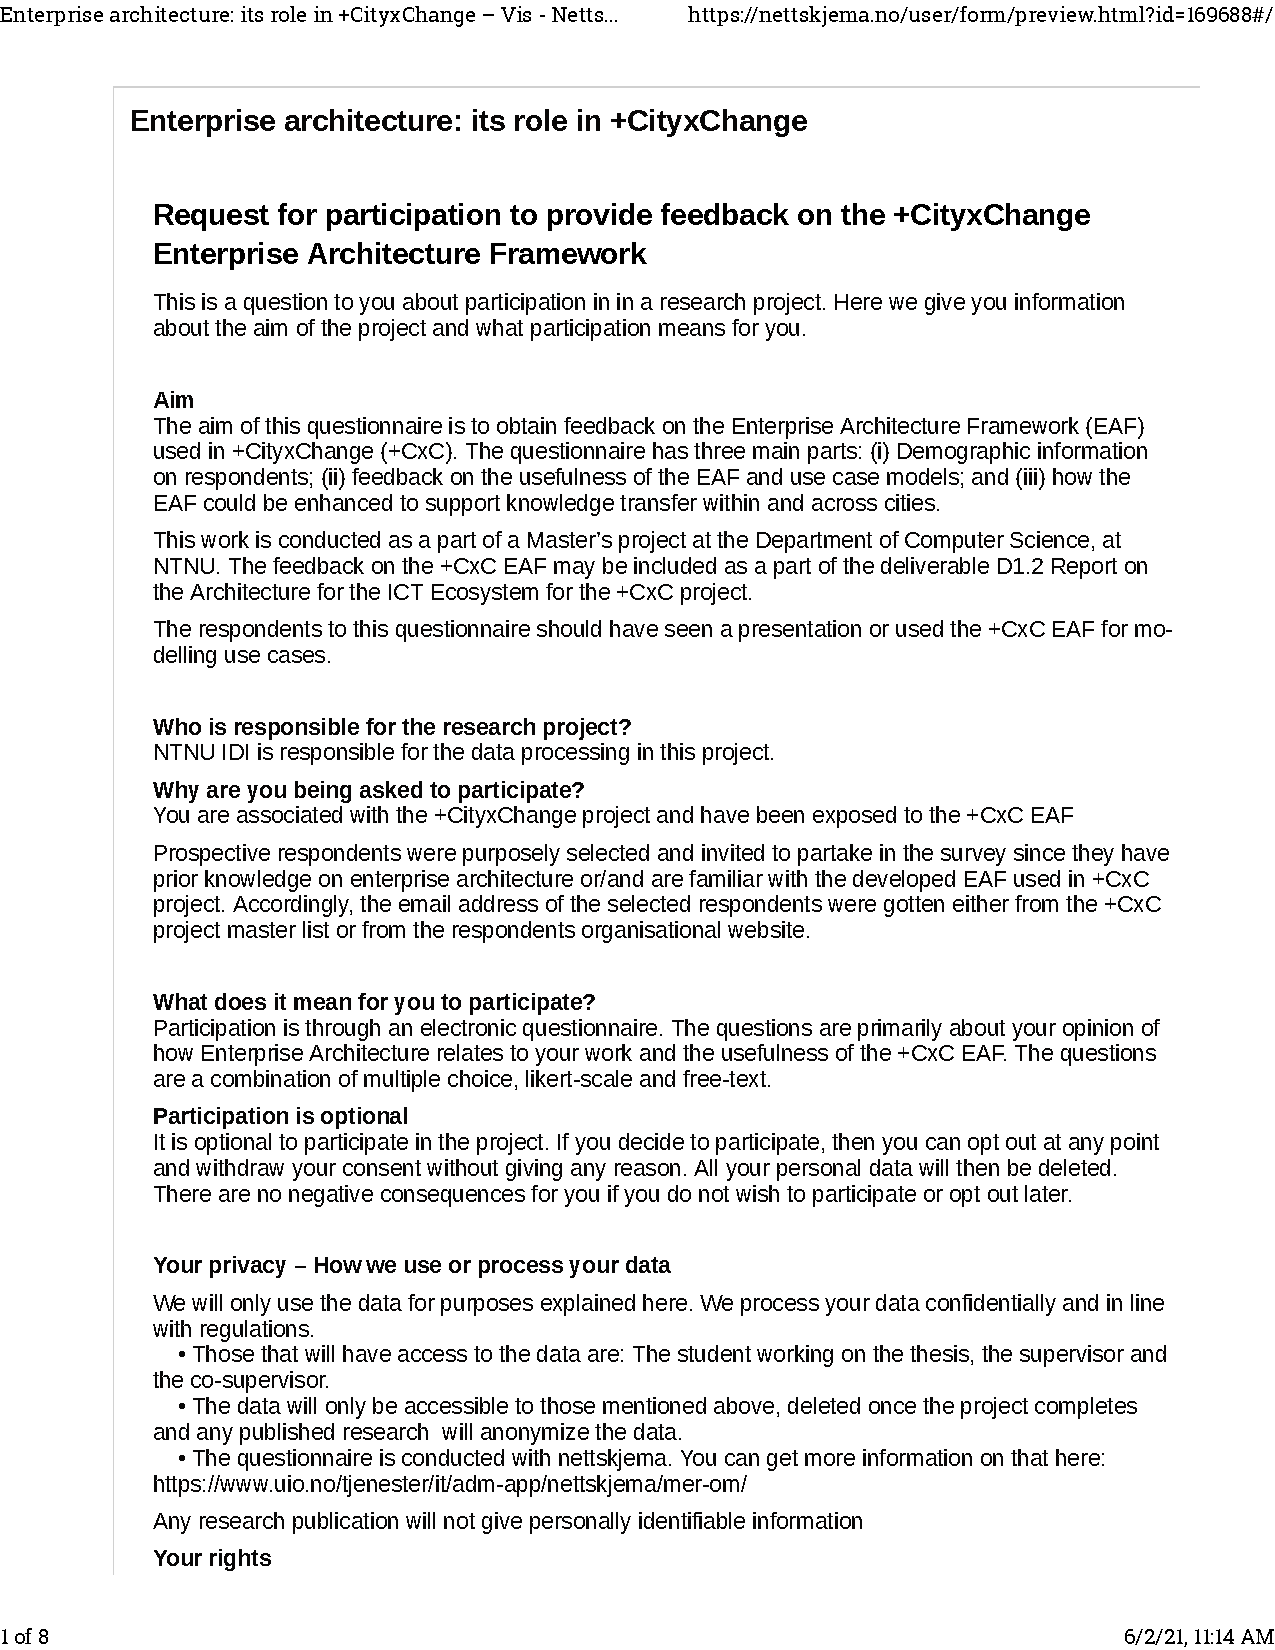
\includepdf[pages=-]{appendices/questionnaire_export.pdf}
%\input{appendices/a-appendix.tex}

\end{document}
